\documentclass[11pt,a4paper]{article}

% ---------------------------------------------------------------------------
% Reliable copying of chemical states: finite-molecule guarantees and
% molecular redundancy.
%
% Author metadata: set the three macros below before submission.
% ---------------------------------------------------------------------------
\newcommand{\PaperAuthor}{Author name to be inserted}
\newcommand{\PaperAffiliation}{Affiliation to be inserted}
\newcommand{\PaperDate}{13 September 2026}

\usepackage[T1]{fontenc}
\usepackage[utf8]{inputenc}
\usepackage{lmodern}
\usepackage{microtype}
\usepackage[a4paper,margin=1.05in]{geometry}
\usepackage{amsmath,amssymb,amsthm,mathtools}
\usepackage{booktabs}
\usepackage{array}
\usepackage{longtable}
\usepackage{enumitem}
\usepackage{xcolor}
\usepackage{tikz}
\usetikzlibrary{arrows.meta,positioning,fit,calc,shapes.geometric}
\usepackage{pgfplots}
\pgfplotsset{compat=1.18}
\usepackage[obeyspaces,spaces]{url}
\usepackage[numbers,sort&compress]{natbib}
\usepackage[colorlinks=true,linkcolor=blue!55!black,citecolor=blue!55!black,urlcolor=blue!55!black]{hyperref}
\hypersetup{pdftitle={Reliable copying of chemical states: finite-molecule guarantees and molecular redundancy},
  pdfkeywords={compositional inheritance, chemical memory, stochastic reaction networks, growth and division, Lyapunov certificates, Lean}}

\DeclareUrlCommand\lean{\urlstyle{tt}}
\setlist{itemsep=2pt,topsep=3pt}
\setlength{\emergencystretch}{1.5em}

\theoremstyle{plain}
\newtheorem{theorem}{Theorem}[section]
\newtheorem{proposition}[theorem]{Proposition}
\newtheorem{lemma}[theorem]{Lemma}
\newtheorem{corollary}[theorem]{Corollary}
\theoremstyle{definition}
\newtheorem{definition}[theorem]{Definition}
\newtheorem{assumption}[theorem]{Assumption}
\theoremstyle{remark}
\newtheorem{remark}[theorem]{Remark}

\newcommand{\R}{\mathbb R}
\newcommand{\N}{\mathbb N}
\newcommand{\PP}{\mathbb P}
\newcommand{\EE}{\mathbb E}
\newcommand{\cL}{\mathcal L}
\newcommand{\cB}{\mathcal B}
\newcommand{\cK}{\mathcal K}
\newcommand{\Bin}{\operatorname{Bin}}
\newcommand{\Pois}{\operatorname{Pois}}
\newcommand{\norm}[1]{\lVert#1\rVert_\infty}
\newcommand{\fall}[2]{(#1)_{#2}}
\newcommand{\Molar}{\mathrm{M}}
\newcommand{\micro}{\mu}
\newcommand{\dd}{\mathrm d}
\DeclareMathOperator{\diag}{diag}

\title{Reliable copying of chemical states:\\ finite-molecule guarantees and molecular redundancy}
\author{\PaperAuthor\\[2pt] {\small\itshape \PaperAffiliation}}
\date{\PaperDate}

\begin{document}
\maketitle

\begin{abstract}
Chemical multistability supplies candidate memory states, but a list of stable states does not say whether a finite population of molecules copies a state reliably through growth, division and recovery. We treat copying as a complete stochastic cycle: an admitted parent must reach division, its molecules must be allocated to two daughters, and both daughters must return to the admitted region of the same label, from which the same guarantee applies again. We prove three separate results and keep their scopes distinct. First, a constructed pair of interacting reversible modules stores four concentration-state labels with at most 874 resident molecules per newborn module; under ideal external pool and volume control, every admitted parent produces two correctly returned daughters at its first division within 20 seconds with probability at least $0.9901$, uniformly over a positive interaction and growth-reversal interval. Second, for $k$ interacting modules satisfying a local quadratic recovery inequality, bounded reaction activity and bounded total incident exchange, the one-generation failure probability is at most $kC(\gamma)e^{-cN}$ with an exponent and an interaction allowance independent of $k$; for an explicit four-species module this gives sufficient copy numbers $N=O(\log(kG/\eta))$ for a designated lineage of $G$ divisions and $O(G+\log(k/\eta))$ for a complete binary family, with matching necessary orders for immediate return of both daughters. Third, the nominal eight-species kinetic model of Semenov et al.\ supports a prescribed split, refill and 500-second recovery protocol at $39.853\,\micro$L with joint daughter return probability at least $0.992$. Uniform return implies repeated copying without any independence assumption between siblings or generations. The proofs combine finite-state generator certificates, exact rational arithmetic, the actual complementary allocation law and state-dependent offspring kernels. The finite-model theorems and the certified-generation kernel are checked in Lean~4; the remaining conventional steps are identified explicitly.
\end{abstract}

\section{Introduction}\label{sec:intro}

A chemical system with several stable compositions can, in principle, store information in the composition it occupies. This idea underlies compositional models of prebiotic heredity \citep{segre2000,vasas2012}, analyses of inheritance in compartmentalized autocatalytic networks under growth and division \citep{matsubara2026,singh2023}, and the question of how many heritable states a chemistry with a given number of species can support \citep{virgo2015}. Bistable and oscillatory networks of small organic molecules have been realized experimentally in flow reactors \citep{semenov2016}. None of this establishes that a \emph{finite} population of molecules copies a stored state reliably, and the gap is not a technicality. Growth changes concentrations and may consume the very species that supports a state. Division allocates molecules at random, and the two daughters are complementary rather than independent. Any recovery after birth takes time and can itself fail. A stable composition is therefore only the starting point; what has to be controlled is the complete cycle.

This paper asks a quantitative version of the question. Under a fully specified stochastic growth-and-division protocol, can both daughters recover the parent's chemical label and become admissible parents themselves, with an explicit probability and an explicit molecular budget? And when more labels must be stored, or more divisions must succeed, how does the required molecular redundancy grow?

\paragraph{Copying as a complete cycle.}
Throughout, a label $\ell$ is represented by an \emph{admitted region} $B_\ell$ of newborn or restart states, chosen so that the copying guarantee is uniform over $B_\ell$. One cycle succeeds when an admitted parent reaches the specified division event within the allowed time and resources, its molecules are distributed to two daughters by the protocol's actual partition law, and both daughters satisfy the same label's admission condition at the protocol's inspection time. Success is deliberately stronger than a decoder assigning the correct label: a daughter can pass a threshold test while lying outside the set on which the next cycle's theorem applies. The reward for this stronger definition is that repeated copying follows by conditioning alone, with no independence assumption between siblings or generations (Section~\ref{sec:events}).

\paragraph{Three results.}
We prove three separate results and keep their scopes distinct; Table~\ref{tab:three} summarizes them.
\begin{enumerate}[label=(\Alph*)]
\item \emph{A small constructed source} (Section~\ref{sec:constructed}). Two interacting reversible two-species modules, coupled through shared consumptive growth and cross-catalysis, store four concentration-state labels with at most $874$ resident molecules in each newborn module. Under an ideal external controller that prescribes the volume and holds two food and two waste pools at fixed activities, every admitted parent produces two correctly returned daughters at its first division within $20$ seconds with probability at least $0.9901$, uniformly over the interaction strength $\epsilon\in[0,0.1]$ and the growth-reversal rate $\rho\in[0,2\times10^{-7}]$, and in particular on a strictly positive rectangle. The proof is a finite-state generator certificate checked in exact integer arithmetic, together with a sharp stopped-counter estimate that makes the complete-cycle reservoir capacity per pool about $0.166$ pmol.
\item \emph{Molecular redundancy for many modules} (Section~\ref{sec:redundancy}). For $k$ interacting modules with $d$ resident species each, sharing consumptive growth and exchanging a growth species through a graph with bounded total incident weight, a local quadratic recovery inequality and bounded reaction activity give a one-generation failure probability at most $kC(\gamma)e^{-cN}$, where $N$ is the birth membrane count per module and the exponent $c$ and interaction allowance do not depend on $k$. For an explicit four-species module the sufficient copy number for a designated lineage of $G$ divisions is $O(\log(kG/\eta))$ at target error $\eta$, and $O(G+\log(k/\eta))$ for a complete binary family. A partition obstruction gives matching necessary orders for immediate return of both daughters, so these orders are sharp for that copying criterion. The constants are astronomically conservative, and the sufficient bound rescales physical rates with $k$; we state exactly which costs the asymptotic statement hides.
\item \emph{A nominal published chemistry} (Section~\ref{sec:semenov}). The eight-species kinetic model reconstructed from Semenov et al.\ \citep{semenov2016}, at its nominal rate constants, supports a prescribed protocol of fair splitting, refilling with fresh feed and $500$ seconds of recovery in a continuously stirred reactor of $39.853\,\micro$L: both daughters return to the same rational return region with probability at least $124/125=0.992$. The certified regions are narrow, the recovery is imposed, and deterministic sensitivity diagnostics show why the theorem must not be read as an experimentally validated uncertainty range.
\end{enumerate}
The conceptual link between the three is reliable return of a label under specified operations. They do not combine into one chemistry that is simultaneously small, experimentally identified and autonomous: the $874$-molecule bound belongs to the constructed source, the logarithmic orders belong to the redundancy theorem's own chemistry, and the Semenov result uses roughly $10^{18}$ active molecules under an external protocol.

\begin{table}[t]
\centering\small
\caption{The three results and their scopes. ``Return'' always means that both daughters lie in the admitted region of the same label; the inspection time differs between protocols.}\label{tab:three}
\begin{tabular}{@{}>{\raggedright\arraybackslash}p{2.6cm}>{\raggedright\arraybackslash}p{3.9cm}>{\raggedright\arraybackslash}p{3.9cm}>{\raggedright\arraybackslash}p{3.9cm}@{}}
\toprule
 & (A) Constructed source & (B) Redundancy theorem & (C) Nominal Semenov model\\
\midrule
Chemistry & two two-species modules, hypothetical reversible rate table, shared growth marker, cross-catalysis & $k$ modules of $d$ species; explicit four-species and two-species instances; growth-species exchange graph & eight tracked species of Semenov et al.\ \citep{semenov2016} in a flow reactor at nominal rates\\
Stored quantity & four concentration-state words $\sigma\in\{0,1\}^2$ & words $\sigma\in\{0,1\}^k$ with a relative-composition readout & two labels, thiol concentration state (relative readout also valid)\\
Resource measure & $\le874$ residents per newborn module; birth marker $N=53$; pools reset by the controller & birth membrane count $N$ per module; $N\ge1.4\times10^{20}$ floor for the four-species instance & $\Omega=2.4\times10^{19}$ molecules per molar, $V=39.853\,\micro$L; feed quota $1.2\times10^{19}$ per daughter\\
Success event & first division by $20$ s, no monitor triggered, both daughters in the boxes at birth & certified generation, or immediate first division, with both daughters in the birth regions & both daughters in the return ellipsoid after split, refill and $500$ s recovery\\
Guarantee & $\ge0.9901$ per cycle, uniform in $\epsilon\in[0,0.1]$, $\rho\in[0,2\times10^{-7}]$ & failure $\le kC(\gamma)e^{-cN}$; $N=\Theta(\log(kG/\eta))$ lineage, $\Theta(G+\log(k/\eta))$ family & $\ge0.992$ per cycle, uniform over the return regions\\
Main limitations & ideal instantaneous pool and volume control; hypothetical compounds & conservative constants; rates rescaled with $k$; deadline $O(k/\gamma)$; necessity only for immediate return & nominal parameters; narrow regions; imposed recovery; known model/data discrepancy\\
Verification & Lean~4, exact integer tables & Lean~4 for the certified kernel and the necessity bound; one conventional transfer lemma & Lean~4, exact rational polynomial certificates\\
\bottomrule
\end{tabular}
\end{table}

\paragraph{What is not claimed.}
None of the results establishes autonomous compartment growth, membrane geometry, selection, differential reproduction, or open-ended evolution; the guarantees concern copying under the stated external operations. The Semenov result is a prediction of a specified nominal model, not an experimental demonstration. Neither result claims to introduce chemical heredity or bistability as topics. We also do not claim that exponential residence at large volume is new; it has general antecedents in large-deviation theory for reaction networks \citep{agazzi2018} and in Lyapunov methods for stochastic reaction networks \citep{gupta2014,kuntz2019}. The contributions are the explicit, uniform finite-copy bounds attached to literal stochastic protocols, the uniformity in the number of modules, and the fact that every quantitative constant is the output of an exactly checked certificate rather than an estimate from simulated trajectories.

\paragraph{Methods.}
All processes are continuous-time Markov jump processes on integer counts with mass-action propensities \citep{gillespie1977,kurtz1972,andersonkurtz2015}. Probabilities of one cycle are bounded by comparison functions on a finite stopped model: a subsolution $v$ of the backward inequality and a nonnegative decaying witness $w$ turn a generator inequality into a deadline bound (Lemma~\ref{lem:deadline}). The comparison functions are proposed numerically and then checked in exact integer or rational arithmetic; for the Semenov model they are time-dependent rational quadratic forms on $38$ polynomial time pieces. Division is handled through the actual complementary binomial allocation, either as an exact terminal payoff or through union bounds, never through a product of sibling probabilities. The passage from finite stopped models to the actual count process uses nonexplosion and a pathwise coupling up to the first monitored event. The finite-model theorems and the certified-generation kernel of the redundancy theorem are checked in Lean~4 with Mathlib \citep{demoura2021,mathlib2020}; Appendix~\ref{app:verification} lists the declarations, the receipts and the exact boundary of what is machine-checked.

\paragraph{Organization.}
Section~\ref{sec:events} defines the copying cycle, offspring kernels and the repeated-copying lemma, and distinguishes a designated lineage from a complete family. Section~\ref{sec:constructed} states and proves the constructed-source theorem. Section~\ref{sec:redundancy} states the general transmission principle, its four-species instance, the immediate-copying bounds and the resulting molecular-redundancy orders. Section~\ref{sec:semenov} treats the nominal Semenov protocol. Section~\ref{sec:discussion} discusses what the results establish and what they leave open. The appendices give the verification map, the four-species source certificates and the Semenov certificate constants.

\section{Copying events, offspring kernels and repeated copying}\label{sec:events}

\subsection{States, labels and admitted regions}
A compartment state consists of the integer count vector $n$ of its resident species, a volume-like variable (a membrane or marker count $m$ in the growth protocols, a fixed volume $V$ in the split--refill protocol), and whatever protocol variables affect the future law (an event counter, a feed inventory). A \emph{label} $\ell$ ranges over a finite set; for $k$ binary modules it is a word $\sigma\in\{0,1\}^k$. Each label has an \emph{admitted region} $B_\ell$, a set of restart states. A \emph{decoder} is a fixed map from states to labels that never inspects the true label; in every protocol below it is a coordinate threshold. Membership in $B_\ell$ is strictly stronger than decoder correctness: $B_\ell$ is the set on which the one-cycle theorem is proved uniformly, and a state that decodes correctly but lies outside $B_\ell$ carries no guarantee for the next cycle.

Which quantity a label measures is part of the statement. In Section~\ref{sec:constructed} the admitted regions are boxes of resident \emph{counts} at a prescribed volume, so the stored quantity is a concentration state (Proposition~\ref{prop:ratio} shows that normalized composition alone does not separate the regions). In Sections~\ref{sec:redundancy} and~\ref{sec:semenov} the regions additionally admit a relative-composition readout.

\subsection{The copying cycle}
\begin{definition}[One copying cycle]\label{def:cycle}
Fix a protocol and a label $\ell$. Starting from an admitted parent $n\in B_\ell$, the cycle \emph{succeeds} when, in chronological order,
\begin{enumerate}[label=(\roman*)]
\item the parent reaches the protocol's division event within the allowed time, without triggering any failure monitor the protocol prescribes (resource quota, domain exit, forbidden event);
\item the resident molecules are assigned to two daughters by the protocol's partition law, and the daughters' volumes and any refill are set as prescribed;
\item both daughters complete the prescribed recovery, if any, and lie in $B_\ell$ at the protocol's inspection time;
\item the state variables needed to run the protocol again are restored by the protocol's label-blind reset, so that daughter A's inspected state is again an admitted parent.
\end{enumerate}
\end{definition}

Two inspection conventions occur. In the growth--division protocols of Sections~\ref{sec:constructed} and~\ref{sec:redundancy}, daughters are inspected \emph{at birth}, immediately after allocation, and the next cycle starts from the birth state; nothing after birth is required. In the split--refill--recovery protocol of Section~\ref{sec:semenov}, daughters are inspected at the end of a fixed recovery interval, and daughter A's terminal state is the next parent. In both cases the inspected state is exactly the state from which the next cycle is run, so no additional residence estimate is needed. Figure~\ref{fig:cycle} shows the cycle.

\begin{figure}[t]
\centering
\resizebox{\linewidth}{!}{%
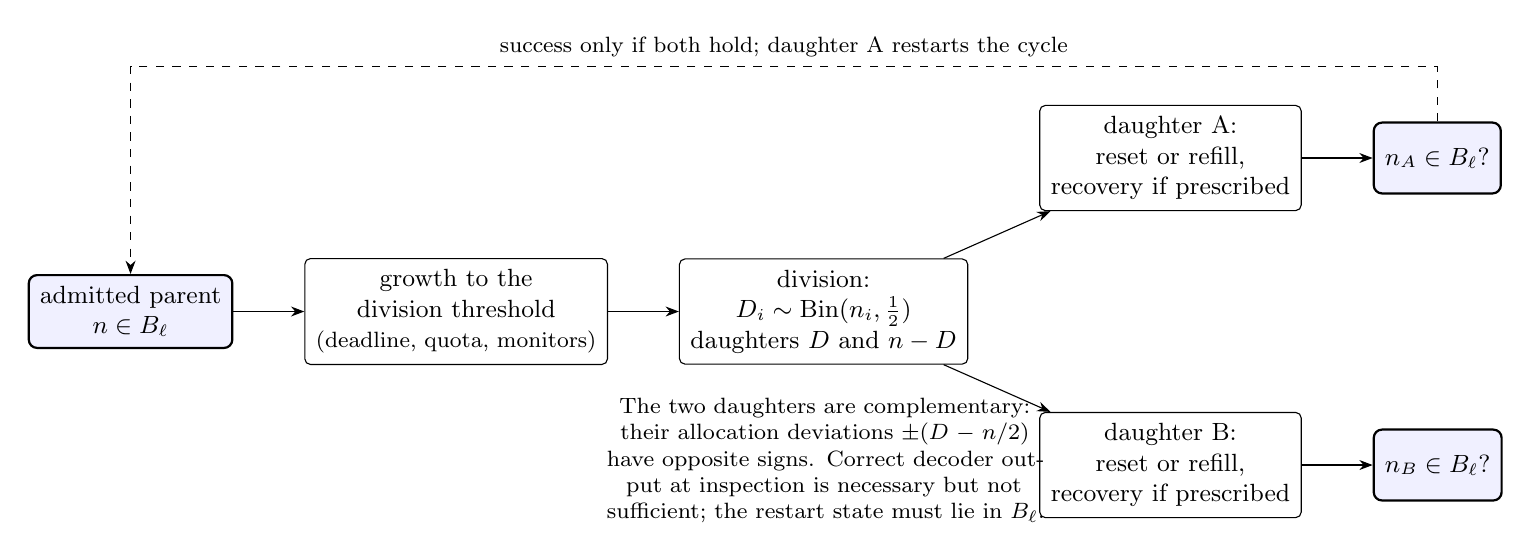
\begin{tikzpicture}[>=Stealth,font=\small,
  box/.style={draw,rounded corners=2pt,align=center,inner sep=4pt,minimum height=9mm},
  reg/.style={draw,thick,rounded corners=3pt,fill=blue!6,align=center,inner sep=4pt,minimum height=9mm},
  lab/.style={font=\footnotesize,align=center}]
\node[reg] (parent) {admitted parent\\ $n\in B_\ell$};
\node[box,right=9mm of parent] (growth) {growth to the\\ division threshold\\ {\footnotesize(deadline, quota, monitors)}};
\node[box,right=9mm of growth] (div) {division:\\ $D_i\sim\Bin(n_i,\tfrac12)$\\ daughters $D$ and $n-D$};
\node[box,above right=2mm and 9mm of div,yshift=4mm] (recA) {daughter A:\\ reset or refill,\\ recovery if prescribed};
\node[box,below right=2mm and 9mm of div,yshift=-4mm] (recB) {daughter B:\\ reset or refill,\\ recovery if prescribed};
\node[reg,right=9mm of recA] (inA) {$n_A\in B_\ell$?};
\node[reg,right=9mm of recB] (inB) {$n_B\in B_\ell$?};
\draw[->] (parent) -- (growth);
\draw[->] (growth) -- (div);
\draw[->] (div) -- (recA);
\draw[->] (div) -- (recB);
\draw[->] (recA) -- (inA);
\draw[->] (recB) -- (inB);
\draw[->,dashed] (inA.north) |- ++(0,7mm) -| node[pos=0.25,above,lab]{success only if both hold; daughter A restarts the cycle} (parent.north);
\node[lab,below=3mm of div,text width=6.2cm] {The two daughters are complementary: their allocation deviations $\pm(D-n/2)$ have opposite signs. Correct decoder output at inspection is necessary but not sufficient; the restart state must lie in $B_\ell$.};
\end{tikzpicture}}
\caption{One copying cycle. Uniform return to $B_\ell$ is proved for every parent in $B_\ell$; a success at daughter A therefore restarts the same guarantee.}\label{fig:cycle}
\end{figure}

\subsection{Offspring kernels and repeated copying}
Let $S_\ell$ denote the set of possible restart states of daughter A (a finite set in all protocols below). One cycle defines a substochastic \emph{offspring kernel}
\[
 K_\ell(n,n')=\PP_n\bigl(\text{cycle succeeds, daughter A's inspected state is }n'\bigr),\qquad n\in B_\ell,\ n'\in S_\ell,
\]
whose missing mass $1-K_\ell(n,S_\ell)$ is the failure probability from $n$. Success forces $n'\in B_\ell$, so $K_\ell(n,S_\ell)=K_\ell(n,B_\ell)$. Because the protocol's reset is label-blind and restores every non-resident variable to its prescribed value, the law of the next cycle depends on the past only through $n'$.

\begin{lemma}[Uniform return implies repeated copying]\label{lem:iteration}
If $K_\ell(n,B_\ell)\ge p$ for every $n\in B_\ell$, then for every $n\in B_\ell$ and $G\ge0$ the probability that all $G$ inspected cycles along the designated daughter-A lineage succeed is at least $p^G$. Writing $p=1-\varepsilon$, it is also at least $\max\{0,1-G\varepsilon\}$.
\end{lemma}
\begin{proof}
Let $S_0\equiv1$ on $B_\ell$ and $S_{g+1}(n)=\sum_{n'\in B_\ell}K_\ell(n,n')S_g(n')$, the probability of $g+1$ successive successes from $n$. If $S_g\ge p^g$ on $B_\ell$ then $S_{g+1}(n)\ge p^g K_\ell(n,B_\ell)\ge p^{g+1}$. The linear bound is Bernoulli's inequality, or a union bound over the $G$ conditional failure events. No independence between generations is used; the multiplication is valid because the conditional guarantee is uniform over the restart set.
\end{proof}

Lemma~\ref{lem:iteration} inspects both daughters at every counted division but follows only daughter A. It says nothing about the other daughter's descendants. For a complete family the number of inspected divisions grows exponentially with the depth.

\begin{proposition}[A designated lineage and an entire family]\label{prop:family}
Let $K_\ell(n,(n_A,n_B))$ be the joint law of both inspected daughter states on success, with $\sum_{(n_A,n_B)}K_\ell(n,(n_A,n_B))\ge p=1-\varepsilon$ for all $n\in B_\ell$. Let $F_G$ be the event that every division in the complete binary family through depth $G$ succeeds, the initial parent being at depth $0$. There are $D_G=2^G-1$ such divisions, and
\[
 \PP_n(F_G)\ge p^{2^G-1}\ge1-(2^G-1)\varepsilon .
\]
\end{proposition}
\begin{proof}
Define $f_0\equiv1$ and $f_{g+1}(n)=\sum_{(n_A,n_B)}K_\ell(n,(n_A,n_B))f_g(n_A)f_g(n_B)$. This is the probability that the family through depth $g+1$ succeeds, constructed with fresh compartment trajectories conditional on the \emph{joint} daughter state; it does not factor the distribution of the sibling compositions. If $f_g\ge p^{D_g}$ on $B_\ell$ then $f_{g+1}\ge p^{2D_g}\,p=p^{D_{g+1}}$, since $D_{g+1}=1+2D_g$. Equivalently, reveal divisions in breadth-first order while all earlier ones have succeeded; each next parent was born admitted, so its conditional success probability is at least $p$, and there are exactly $D_G$ opportunities.
\end{proof}

The terminal generation of the family is inspected with the same convention as in Definition~\ref{def:cycle}: at birth in the growth protocols, after recovery in the split--refill protocol. A one-cycle bound of $0.9901$ gives $0.9901^{10}>0.905$ along ten lineage divisions but only $0.9901^{1023}\approx3.8\times10^{-5}$ for a complete family of depth ten; the family bound is a lower bound and not evidence that most descendants fail.

\subsection{Complementary allocation}\label{sec:partition}
In every protocol below, division allocates each resident molecule independently and fairly to one of the two daughters. Conditional on the parent's count vector $n$, one draws $D_i\sim\Bin(n_i,1/2)$ independently across species and assigns $(D_i,n_i-D_i)$ to daughters A and B. The two daughter vectors are dependent: their deviations from $n/2$ are negatives of each other, and $\operatorname{Cov}(D_i,n_i-D_i)=-n_i/4$. Consequently the probability that both daughters return is \emph{not} the product of the two marginal return probabilities. Two devices replace that product. In Section~\ref{sec:constructed} the joint return probability is an exact finite binomial sum and is used as the terminal payoff. In Sections~\ref{sec:redundancy} and~\ref{sec:semenov} the daughters' deviations are bounded by a common event (a sup-norm tail, or a union bound over the two marginals); the reflection $d\mapsto n-d$ shows that daughter B has the same marginal law as daughter A, so one marginal estimate serves both.

\begin{remark}[What uniformity must include]
The restart set must contain every variable that can change the future law. In the constructed source the controller resets the food, waste and marker pools and the event counter at each division, without inspecting the label or touching the resident counts; in the Semenov protocol the feed quota is renewed each cycle. In both cases the restart state is the resident count vector alone, and the bounds of Theorems~\ref{thm:constructed} and~\ref{thm:semenov} are uniform over it. A bound uniform only in resident concentration would not justify another generation if a depleted reservoir or a controller phase were carried across cycles; we therefore charge the reservoir explicitly (Proposition~\ref{prop:capacity}) and state where fresh resources enter.
\end{remark}

\section{A small constructed source with two interacting modules}\label{sec:constructed}

This section gives the first result: a hypothetical but fully specified chemistry that copies four concentration-state labels with at most $874$ resident molecules per newborn module. The mechanism is deliberately small so that its one-cycle probability can be certified in exact integer arithmetic on a finite state space. Its physical assumptions are equally explicit: an ideal external controller prescribes the volume, holds food and waste pools at fixed activities, and resets those pools at division without inspecting the stored label.

\subsection{Chemistry}\label{sec:chem}
There are two resident modules $i=0,1$, each with two resident species $X_i,Y_i$, a shared growth marker with count $m$, and, for each module, a controlled food pool $F_i$ and a controlled waste pool $W_i$. The resident reactions of each module are
\begin{equation}\label{eq:resident}
 F\rightleftharpoons X,\qquad Y+F\rightleftharpoons2X,\qquad
 2X\rightleftharpoons X+Y,\qquad X+Y\rightleftharpoons Y+W,\qquad X\rightleftharpoons W.
\end{equation}
Read chemically: food is converted to $X$ directly and, autocatalytically, by $Y$; two $X$ molecules convert one of them to $Y$; $Y$ catalyses the degradation of $X$ to waste; and $X$ leaks to waste. Every reaction is reversible. At the maintained food and waste activities the effective count propensities are those of Table~\ref{tab:rates}; repeated reactants use falling factorials with no additional factorial divisor, so $2X\to X+Y$ has propensity $15x(x-1)/m$.

\begin{table}[t]
\centering
\caption{Effective propensities per module in model time. $x,y$ are the module's resident counts and $m$ is the shared marker count, which also sets the volume. The reverse coefficients are chosen so that the effective ratios $K_{FX}=150000$, $K_{YX}=1$ and $K_{XW}=100000$ are consistent around every cycle of \eqref{eq:resident}; these define a hypothetical chemistry.}\label{tab:rates}
\begin{tabular}{@{}lll@{}}\toprule
Reaction pair & Forward propensity & Reverse propensity\\\midrule
$F\rightleftharpoons X$ & $(193/5)\,m$ & $(193/750000)\,x$\\
$Y+F\rightleftharpoons2X$ & $1555\,y$ & $(311/30000)\,x(x-1)/m$\\
$2X\rightleftharpoons X+Y$ & $15\,x(x-1)/m$ & $15\,xy/m$\\
$X+Y\rightleftharpoons Y+W$ & $100\,xy/m$ & $y/1000$\\
$X\rightleftharpoons W$ & $(105/2)\,x$ & $(21/40000)\,m$\\\bottomrule
\end{tabular}
\end{table}

The modules interact in two ways. Each module contributes to growth through $X_i\to M$ at propensity $x_i/10$: one resident molecule is consumed and the shared marker $m$ increases by one, which dilutes both modules. The reverse channel $M\to X_i$ has propensity $\rho m$. Cross-catalysis $X_i+Y_j\rightleftharpoons Y_i+Y_j$ for $j\ne i$ has propensities $\epsilon x_iy_j/m$ forward and $\epsilon y_iy_j/m$ backward. The two parameters $\epsilon\ge0$ and $\rho\ge0$ are the interaction strength and the growth-reversal rate; the theorem below is uniform over an interval of each.

Assigning equal positive masses to $F,X,Y,W$ and $M$ makes every displayed reaction mass-balanced. The imposed food-to-waste affinity at the stipulated pool activities is $\log(K_{FX}K_{XW})=\log(1.5\times10^{10})\simeq23.43$ in units of $k_BT$. This is the driving affinity of the reservoir pair, not a dissipation per copied bit.

\paragraph{Dimensional calibration.}
Take a concentration scale $C_0=1\,\micro\Molar$, one second per model-time unit, and food and waste concentrations $1000\,C_0$. The controller prescribes the volume $V=m/(N_AC_0)$ and holds each local pool at $1000\,m$ molecules after every event. A newborn has $m=N=53$, corresponding to a volume of about $0.0880$\,fL, and divides at the first arrival at $m=2N=106$. The corresponding physical rate table has, for example, $Y+F\to2X$ at $1.555\times10^6\,\Molar^{-1}\mathrm s^{-1}$ at $1$\,mM food and $X\to W$ at $52.5\,\mathrm s^{-1}$. The marker is a chemical growth product coupled to the prescribed volume; it is not asserted to be a membrane, and exact instantaneous pool adjustment, prescribed volume and well-mixed equal-volume division are assumptions of the protocol rather than consequences of the chemistry.

\subsection{Protocol, regions and the theorem}\label{sec:protocol}
The protocol counts every model event, including an auxiliary rate-one self-event that keeps the total jump rate positive, and rejects the cycle when the counter reaches the quota $J=10^8$. It monitors exits from the certified resident domain $\{x_i\le16m,\ y_i\le4m\}$ and every reverse-growth event; both are counted as failure. At division, the residents of each module undergo the complementary allocation of Section~\ref{sec:partition}. The controller then sets each daughter's marker to $53$ and each local pool to $53000$ molecules, without changing the allocated resident counts or inspecting the label.

At birth the admitted boxes of the two labels are
\begin{equation}\label{eq:boxes}
 B_0=\{6\le x\le106,\ 0\le y\le8\},\qquad B_1=\{371\le x\le742,\ 6\le y\le132\},
\end{equation}
with integer counts. A word $\sigma\in\{0,1\}^2$ means $(x_i,y_i)\in B_{\sigma_i}$ for both modules, so the admitted region of the word is $B_\sigma=B_{\sigma_0}\times B_{\sigma_1}$. The decoder is the threshold $x>212$, applied to each module separately. The preparations $(53,0)\in B_0$ and $(530,53)\in B_1$ show that every word has admitted states. A newborn module in $B_1$ has at most $742+132=874$ resident molecules, and one in $B_0$ at most $114$.

\begin{theorem}[Finite-drive concentration-state copying]\label{thm:constructed}
For the quota-controlled source above, every admitted newborn of every word has probability at least $0.9901$ of first division by $T=20$ with both complementary daughters returned to the same word's admitted boxes and no monitor triggered. This holds uniformly for
\[
 0\le\epsilon\le0.1,\qquad0\le\rho\le2\times10^{-7},
\]
in particular on the strictly positive rectangle $10^{-4}\le\epsilon\le0.1$, $10^{-7}\le\rho\le2\times10^{-7}$. Each newborn module has at most $874$ resident molecules. Ten inspected lineage cycles succeed with probability at least $0.9901^{10}>0.905$.
\end{theorem}

The success event is Definition~\ref{def:cycle} with inspection at birth: the restart state of daughter A is its birth count vector, and the marker, pools and counter are reset by the controller. The first actual division can be preceded by histories that the conservative monitors reject; the theorem bounds the probability of the monitored successful subset, which is contained in the event ``first division by $T$ with both daughters in $B_\sigma$''. The last sentence is Lemma~\ref{lem:iteration}.

\subsection{The proof: a finite generator certificate}\label{sec:certificate}
For a finite jump model with channels $r$, propensities $a_r(z)$ and jumps $\nu_r$, write
\[
 \cL f(z)=\sum_r a_r(z)\bigl(f(z+\nu_r)-f(z)\bigr).
\]
The following comparison converts generator inequalities into a deadline bound. It is the only probabilistic tool needed for the constructed source.

\begin{lemma}[Deadline comparison]\label{lem:deadline}
Let $Z$ be a finite-state jump process with generator $\cL$, and let $h,v,w$ be functions on its state space with $v\le h+w$, $w\ge0$. If $\cL v\ge-\delta$ and $\cL w\le-sw+\eta$ with $s>0$, $\eta\ge0$, then for every state $n$ and $T\ge0$,
\begin{equation}\label{eq:deadline}
 \EE_n h(Z_T)\ \ge\ v(n)-T\delta-e^{-sT}w(n)-\eta/s.
\end{equation}
\end{lemma}
\begin{proof}
On a finite state space $u(t)=\EE_nv(Z_t)$ is differentiable with $u'(t)=\EE_n\cL v(Z_t)\ge-\delta$, so $\EE_nv(Z_T)\ge v(n)-T\delta$. Likewise $g(t)=\EE_nw(Z_t)$ satisfies $g'\le-sg+\eta$, and Gr\"onwall's inequality gives $g(T)\le e^{-sT}w(n)+\eta/s$. Subtracting, $\EE_nh(Z_T)\ge\EE_nv(Z_T)-\EE_nw(Z_T)$ gives \eqref{eq:deadline}. The finite law may be realized by uniformization or by the matrix exponential; the identity $u'=\EE\cL v$ holds for either.
\end{proof}

\paragraph{Local certificates with the other module as a control.}
The state of the pair has four resident coordinates and the marker; a direct backward solve on the joint space is unnecessary. Instead, for each module and each label, rational backward certificates are computed on the volume layers $m=53,\dots,106$ with proposal caps $x\le16m$, $y\le4m$. The other module's influence, its cross-catalytic propensity and its contribution to growth, enters the local generator through affine controls whose ranges are the admissible values on the other module's certified domain. Checking the control extremes covers every admissible neighbouring state, so the local computation makes no independence assumption; it is a worst case over the other module.

Let $h_i$ be the exact terminal payoff of module $i$ at $m=106$: the probability, under complementary allocation of that module's residents, that both daughters' module-$i$ counts lie in $B_{\sigma_i}$, an exact finite binomial sum. Let $h=h_0h_1$ be the joint payoff, which is exactly the probability that both daughters return. Combine the local certificates as
\[
 v=v_0+v_1-1,\qquad w=w_0+w_1 .
\]
This is valid because $h_0+h_1-1\le h_0h_1$ for $h_0,h_1\in[0,1]$, so $v\le h+w$ follows from the local inequalities $v_i\le h_i+w_i$, and the generator of the sum is controlled by the local generators evaluated at the control extremes. Exact exit comparisons handle joint killing: an exit of either module kills the pair, and the local certificates are compared with zero continuation at their own exits.

The checked integer rows establish, for every state of the finite model,
\begin{align}
 v&\le1,& w&\ge0,& v&\le h+w,\label{eq:cert1}\\
 \cL v&\ge-2\times10^{-6},& \cL w&\le-\tfrac58w+\tfrac1{50000},\label{eq:cert2}
\end{align}
and at every admitted newborn $n$ the birth row
\begin{equation}\label{eq:birthcert}
 500000\,v(n)-2\,w(n)\ \ge\ 495550 .
\end{equation}
The numerically proposed certificate is not assumed correct: every row of \eqref{eq:cert1}--\eqref{eq:birthcert} is an integer inequality on exact rational data (about $2.2\times10^7$ transient rows), and the terminal payoffs are exact binomial sums. Appendix~\ref{app:verification} states the trust boundary of the arithmetic.

\paragraph{Pre-monitor bound.}
Apply Lemma~\ref{lem:deadline} with $T=20$, $\delta=2\times10^{-6}$, $s=5/8$, $\eta=1/50000$. Since $e^{-sT}=e^{-25/2}\le1/250000$, \eqref{eq:birthcert} gives $v(n)-e^{-sT}w(n)\ge0.9911$, and hence
\[
 \EE_nh(Z_T)\ \ge\ 0.9911-20\cdot2\times10^{-6}-\tfrac{8}{5}\cdot\tfrac1{50000}=0.991028\ \ge\ 0.991 .
\]

\paragraph{Reverse-growth monitor.}
Every reverse-growth event $M\to X_i$ is rejected. Before division $m\le2N$, so the combined hazard of the two reverse channels is at most $2\rho\cdot2N=4\rho N$, and the probability that such an event occurs by $T=20$ is at most $80\rho N\le0.000848$ at $\rho=2\times10^{-7}$. Killing at these events lowers the generator of $v$ by at most the hazard, since $v\le1$ and the killed continuation is $0\ge v-1$; it can only improve the nonnegative witness $w$. No new backward solve is needed.

\paragraph{Event quota.}
The total event rate of the stopped model, including the self-event and the monitored reverse channels, is at most $\Lambda=4\times10^6$ on the certified domain; rates after an already failed exit are immaterial because the process is frozen there.

\begin{lemma}[Stopped exponential counter bound]\label{lem:quota}
Let $C_t$ count all events of a finite jump process whose total intensity is at most $\Lambda$, stopped at the quota $J$, with $C_0=0$. For every $a\ge1$,
\begin{equation}\label{eq:tail}
 \PP(C_T=J)\le a^{-J}\exp\bigl(\Lambda(a-1)T\bigr).
\end{equation}
For $\Lambda=4\times10^6$, $T=20$, $J=10^8$ and $a=1+10^{-6}$ the right side is at most $2\times10^{-7}$.
\end{lemma}
\begin{proof}
Put $f(c)=a^c/a^J$. Before exhaustion, $\cL f=\lambda(z)(a-1)f\le\Lambda(a-1)f$, where $\lambda(z)$ is the total intensity, and at exhaustion the generator vanishes, so the inequality persists. Gr\"onwall for the finite law gives $\EE f(C_T)\le e^{\Lambda(a-1)T}/a^J$, and $\mathbf1_{\{C_T=J\}}\le f(C_T)$ proves \eqref{eq:tail}, including state-dependent intensities and self-events. For the constants: Bernoulli's inequality gives $a^{10000}\ge1.01$, exact rational arithmetic gives $1.01^{100}\ge2.7$, hence $a^{10^8}\ge2.7^{100}$; with $e<11/4$, $e^{80}/a^{10^8}\le(11/4)^{80}/2.7^{100}<2\times10^{-7}$.
\end{proof}

To attach the quota to the copying bound, lift $v$ unchanged to the state augmented by the counter, including the frozen exhausted states; its drift lower bound is preserved. Set $w$ to zero at exhaustion; its upper drift bound is preserved. The cover inequality $v\le h+w$ then holds with $h$ replaced by $h+\mathbf1_{\{C=J\}}$, because $v\le1$. Applying \eqref{eq:deadline} to the augmented model and subtracting Lemma~\ref{lem:quota} gives the actual quota-controlled payoff
\[
 0.991-0.000848-0.0000002=0.9901518>0.9901 .
\]
The same finite model, with its monitors and quota, is the one whose first-division output defines the offspring kernel; Lemma~\ref{lem:iteration} then gives the ten-cycle statement and completes the proof of Theorem~\ref{thm:constructed}.

\subsection{Resource accounting}\label{sec:resources}
The $874$-molecule figure counts residents of one newborn module. The other inventories are part of the protocol and are charged separately.

\begin{proposition}[Complete-cycle reservoir capacity]\label{prop:capacity}
Each event changes a local pool and the marker by at most one molecule, so restoring a pool to $1000\,m$ after an event requires at most $1001$ supplied or removed molecules. Including startup of the pool at $1000N$, the reset of both daughters' pools after an arbitrary complementary allocation, and decommissioning, a conservative gross supply capacity and a conservative gross disposal capacity per food or waste pool and per cycle are each
\begin{equation}\label{eq:capacity}
 4000N+1001J=100{,}100{,}212{,}000\ \text{molecules}\approx0.1662\ \mathrm{pmol}.
\end{equation}
Four pools over ten inspected cycles need about $6.65$\,pmol of capacity. The marker allowance for startup, reset and removal is $4N=212$ molecules per cycle. The initial local inventory is $213{,}801$ molecules: at most $1748$ residents, $212{,}000$ food and waste molecules, and $53$ marker molecules.
\end{proposition}
\begin{proof}
If a pool with parent count $2q$ is split as $(a,2q-a)$, restoring both daughters to $q$ needs at most $q$ supplied and $q$ removed molecules; with $q=1000N$ this is the $2\cdot1000N$ reset term, and startup and decommissioning contribute $1000N$ each. Every counted event contributes at most $1001$, and there are at most $J$ events per cycle. The identities are checked in Lean (Appendix~\ref{app:verification}).
\end{proof}

These are worst-case capacities, not estimates of consumption. Compared with a crude linear exhaustion estimate, which would require a quota of $2\times10^{12}$ for the same probability loss, Lemma~\ref{lem:quota} reduces the conservative capacity by a factor of about $2\times10^4$. Finite capacity is compatible with the construction; it does not establish that the ideal controller is physically realizable.

\subsection{What the labels measure}\label{sec:ratio}
The decoder $x>212$ is a count threshold at the prescribed birth volume, so it distinguishes concentration states. It is natural to ask whether the labels are also distinguished by the resident composition alone, that is, by the normalized proportions $x:y$. They are not.

\begin{proposition}[Concentration memory, not ratio memory]\label{prop:ratio}
The states $(10,1)\in B_0$ and $(400,40)\in B_1$ have identical normalized resident compositions. Hence no decoder depending only on the proportions of $X$ and $Y$ separates all admitted low states from all admitted high states.
\end{proposition}
\begin{proof}
$(400,40)=40\cdot(10,1)$, and both points satisfy \eqref{eq:boxes}.
\end{proof}

Proposition~\ref{prop:ratio} leaves Theorem~\ref{thm:constructed} intact and fixes its interpretation: the constructed source stores which of two concentration states each module occupies at the controlled volume. An externally controlled reference pool does not change this. The Semenov regions of Section~\ref{sec:semenov} and the redundancy construction of Section~\ref{sec:redundancy} do admit a relative-composition readout; the difference lies in the geometry of the admitted regions, not in the copying theorem.

\section{Molecular redundancy for many interacting modules}\label{sec:redundancy}

The constructed source of Section~\ref{sec:constructed} has two modules and fixed constants. This section asks how the required molecular redundancy grows when $k$ modules must be copied and $G$ divisions must succeed. The chemistry is different from Section~\ref{sec:constructed}: growth is consumptive with a membrane count rather than a controlled marker, there are no external pools to reset, and the interaction is exchange of a growth species through a graph. The answer is a uniform transmission principle: once local reaction quality is fixed, there are a positive exponent, a growth allowance and an interaction allowance that serve every $k$, every admissible exchange graph, every word and every admitted newborn.

\subsection{Model}\label{sec:redmodel}
There are $k\ge1$ disjoint modules, each with $d$ resident species. The count state is $(n,m)$ with $n_{ia}\in\N$ for module $i$ and species $a$, and a common positive integer membrane count $m$, which is the physical volume. A newborn has $m=kN$ and divides at the first time $m=2kN$; both daughters receive $kN$ membrane units, and the residents are allocated complementarily as in Section~\ref{sec:partition}, independently across all molecules. Reaction clocks after birth are fresh conditional on the newborn state.

A resident reaction $\ell$ of module $i$ has consumption and production vectors $\alpha_{i\ell},\beta_{i\ell}\in\N^d$, order $r_{i\ell}=\sum_a\alpha_{i\ell a}$, net change $\nu_{i\ell}=\beta_{i\ell}-\alpha_{i\ell}$ and reference coefficient $c_{i\ell}\ge0$. Its physical propensity is
\begin{equation}\label{eq:physical}
 c_{i\ell}\,k^{r_{i\ell}-2}\,m^{1-r_{i\ell}}\prod_a\fall{n_{ia}}{\alpha_{i\ell a}},
\end{equation}
with falling factorials $\fall{n}{r}=n(n-1)\cdots(n-r+1)$ and no factorial divisor. The designated growth species $z$ is converted into membrane at physical propensity $\gamma n_{iz}/k$, changing $(n_i,m)$ to $(n_i-e_z,m+1)$: growth consumes a resident molecule and dilutes every module. Directed exchange $i\to j$ transfers one $z$ molecule at propensity $w_{ij}n_{iz}/k$, where
\begin{equation}\label{eq:graph}
 w_{ij}=w_{ji}\ge0,\qquad w_{ii}=0,\qquad\sum_jw_{ij}\le\kappa .
\end{equation}
The restriction is on the total incident exchange at a module, not on the graph size: a path or ring with edge weight $\kappa/2$ is admissible for every $k$ (Corollary~\ref{cor:degree}), whereas a complete graph with a fixed edge weight is not.

The analysis uses the rescaled coordinates $v=m/k\in[N,2N]$, $u_i=n_i/v$ and time $\tau=t/k$; in these coordinates the resident propensity per unit $\tau$ is $c_{i\ell}v^{1-r_{i\ell}}\prod_a\fall{n_{ia}}{\alpha_{i\ell a}}$ and the physical concentration is $u_i/k$. These are choices of the theorem: the model has $dk$ species, \eqref{eq:physical} rescales physical coefficients with $k$, and a certified generation lasts at most $k(t_0+t_1)=O(k/\gamma)$ in physical time. Section~\ref{sec:orders} returns to what this means.

\paragraph{Regions and two success events.}
For each word $\sigma\in\{0,1\}^k$, module $i$ has a centre $a_i^\sigma$ and a positive quadratic form $E_i^\sigma(y)=Q_i^\sigma(y,y)$; with birth energy $b$ the closed newborn region is
\begin{equation}\label{eq:birthregion}
 \cB_\sigma(N)=\{n:\ E_i^\sigma(n_i/N-a_i^\sigma)\le b\ \text{for every }i\}.
\end{equation}
A \emph{certified generation} remains in an outer energy tube until a deterministic recovery time $t_0$ (in $\tau$ units), has not divided by $t_0$, is inside an inner recovery region at $t_0$, then remains in a smaller parent tube until division within a further $t_1$ units, and both daughters lie in $\cB_\sigma(N)$. Leaving either tube fails the certificate irreversibly even if later chemistry would repair it. An \emph{immediate successful division} requires only that the first actual division occurs and both daughters lie in $\cB_\sigma(N)$; nondivision counts as failure and repair after birth does not count. Write $A_G$ for immediate success at all $G$ divisions along a designated daughter, both daughters inspected each time, and $F_G$ for immediate success at every division of the complete binary family through depth $G$.

\subsection{The uniform transmission principle}\label{sec:general}
All constants below are fixed before $k$, the graph, the word and $N$; sup norms are used throughout, and module indices are suppressed on local quantities.

\begin{assumption}[Local quality]\label{ass:local}
\begin{enumerate}[label=(H\arabic*)]
\item \emph{Geometry.} $c_0\norm y^2\le Q(y,y)$ and $|Q(y,h)|\le L\norm y\norm h$. There are $M,\lambda,\rho>0$ and levels $M\rho<h_{\rm rec}<h_{\rm par}<b<h_{\rm out}\le c_0R_0^2$. Centres are nonnegative and at most $C-R_0$ coordinatewise for a fixed integer cap $C$, and a fixed readout threshold separates each centre from the opposite label by at least $R_0$.
\item \emph{Local drift.} On every outer product domain, each displacement $y=u-a$ admits $r\in[0,r_{\max}]$ with $\norm y\le r$, $\norm u\le U$, $E(y)\le Mr^2$, and
\[
 2Q\bigl(y,f(u)\bigr)\le-\lambda r^2,\qquad |Q(y,\nu_\ell)|\le Pr,\qquad |Q(\nu_\ell,\nu_\ell)|\le R_1,\qquad f(u)=\sum_\ell c_\ell u^{\alpha_\ell}\nu_\ell,
\]
uniformly over all admissible integer states, not only at the centres.
\item \emph{Activity and finite-volume bias.} $\sum_\ell c_\ell U^{r_\ell}\le A$ and $\sum_\ell c_\ell r_\ell^2(U+1)^{r_\ell}\norm{\nu_\ell}\le D_0$; the second bound controls the discrepancy between falling-factorial rates and fluid monomials by $D_0/v$.
\item \emph{Growth and interaction.} On the outer domains $0<\ell_0\le u_{iz}\le Z$, and $w$ satisfies \eqref{eq:graph}.
\end{enumerate}
\end{assumption}

\begin{theorem}[Uniform certified transmission]\label{thm:general}
Under Assumption~\ref{ass:local} there exist $\gamma_0,\kappa_0,c_*>0$, $N_0<\infty$ and $t_0>0$, independent of $k$, $N$, $w$ and $\sigma$, such that for every $0<\gamma\le\gamma_0$, with $t_1=11/(10\gamma\ell_0)$, every architecture with row sums at most $\kappa_0$, every $N\ge N_0$, every word and every integer newborn in its closed birth region, the certified-generation kernel satisfies
\begin{equation}\label{eq:generalerror}
 K_{\rm cert}(n,\mathrm{failure})\le\varepsilon=kC_*(\gamma)e^{-c_*N},\qquad
 C_*(\gamma)=7+2d+\frac{\lambda\rho}2\Bigl(\frac{t_0}{h_{\rm out}-b}+\frac{t_1}{h_{\rm par}-h_{\rm rec}}\Bigr).
\end{equation}
The integer birth regions are nonempty and have distinct word readouts. Along a designated lineage the certified success probability over $G$ generations is at least $1-G\varepsilon$, and at least $(1-\varepsilon)^G$ when $\varepsilon\le1$.
\end{theorem}

\begin{proof}[Proof sketch]
The proof has three parts; Appendix~\ref{app:source} gives the constants for the explicit source.

\emph{Shared growth cancels correctly.} At a growth event in module $j$, module $i$ sees the jump $\Delta u_i=-(u_i+k\mathbf1_{\{i=j\}}e_z)/(m+1)$. Summing over $j$ with propensities $\gamma vu_{jz}$ before estimating gives the limiting growth force $-\gamma u_{iz}e_z-\gamma\bar u_zu_i$ with $\bar u_z=k^{-1}\sum_ju_{jz}$: consumption plus dilution by shared growth. For the quadratic variation the single consuming jump has size at most $(U+k)/(m+1)$ and the other $k-1$ jumps at most $U/(m+1)$, so the total is at most $\gamma Z(U+1)^2/v$, with no factor $k$. Exchange contributes a force of size at most $2Z\kappa$ and quadratic variation at most $2Z\kappa/v$; incoming and outgoing events both contribute variance. These two estimates are the dimension-uniform heart of the proof.

\emph{Exponential control.} Let $V_i=\exp(\alpha NE_i)$ with the birth copy number $N$ in the exponent. The identity $E_i(y+h)-E_i(y)=2Q_i(y,h)+Q_i(h,h)$ and $e^s-1\le s+s^2$ for $|s|\le1$ reduce every jump to (H1)--(H3) and give, for uniform constants $F,K,B_1,C_1$ built from $A,P,R_1,D_0,L,Z,\gamma,\kappa$,
\[
 \frac{\cL V_i}{\alpha V_i}\le-\lambda Nr^2+NFr+K+\alpha NB_1r^2+\frac{\alpha C_1}N .
\]
Choose $\alpha$ with $\alpha B_1\le\lambda/4$, then small $\gamma_0,\kappa_0$ and large $N_0$ so that $F^2\le\lambda^2\rho/8$ and $K+\alpha C_1/N\le\lambda N\rho/8$; Young's inequality gives $\cL V_i\le\alpha N(-\tfrac\lambda2r^2+\tfrac{\lambda\rho}4)V_i$, negative outside $r^2<\rho$ with rate at least $\alpha\lambda N\rho/4$ and bounded inside. Neither the exponent nor $\kappa_0$ shrinks with $k$.

\emph{Six errors.} A nonnegative test function with generator at most $\beta$ gives $\EE V(X_{t\wedge\tau})\le V(X_0)+\beta t$, and at first exit through energy $h$ its value is at least $e^{\alpha Nh}$; this bounds each tube exit by an energy-gap exponential times $(1+\lambda\rho t/(2g))$, summed over $k$ modules. The affine drift inequality with killing at the outer exit gives recovery to $h_{\rm rec}$ by $t_0=1+4b/(\lambda\rho)$ up to $3ke^{-\alpha N(h_{\rm rec}-M\rho)}$. Early division before $t_0$ has probability at most $e^{-kN/125}$ when $\gamma_0Zt_0\le2/5$, and late division after $t_1$ at most $e^{-9kN/4000}$, by the exponential generating function of the bounded-intensity membrane counter. At division, choose $r_{\rm par}$ and $\delta$ with $h_{\rm par}\le c_0r_{\rm par}^2$ and $h_{\rm par}+2Lr_{\rm par}\delta+L\delta^2<b$: if the sup norm of the allocation deviation $(D-n/2)/N$ is below $\delta$, the quadratic identity puts \emph{both} daughters in the birth region, since their deviations are opposite; a fair-binomial tail and a union bound over $kd$ coordinates give $2kde^{-N\delta^2/C}$. No product over the two daughters is used. Adding outer exit, early division, failed recovery, parent-tube exit, late division and failed partition gives \eqref{eq:generalerror} with constant terms $1+1+3+1+1+2d$. Coordinatewise rounding of the centres gives integer newborns once $N_0$ absorbs the rounding error, and Lemma~\ref{lem:iteration} gives the lineage statement.
\end{proof}

\begin{corollary}[Bounded-degree graphs]\label{cor:degree}
If a symmetric graph has maximum degree at most $\Delta\ge1$ and edge weights at most $\kappa_0/\Delta$, it satisfies the interaction condition of Theorem~\ref{thm:general}. In particular paths and rings admit the fixed positive edge weight $\kappa_0/2$ for every $k$.
\end{corollary}

\subsection{An explicit four-species module}\label{sec:fourspecies}
The resident species are $A,B,z,H$ with the thirteen directed channels of Table~\ref{tab:fourspecies}. Growth consumes $z$ and exchange transfers $z$. The fluid drift is
\begin{equation}\label{eq:fluid}
\begin{aligned}
 \dot A&=6-2A+zB+2e(B-A^2),&\dot B&=27+A-(1+z)B-e(B-A^2),\\
 \dot z&=A-Bz-16z-4z^2+3H,&\dot H&=16z+2z^2-(2+d_0)H,
\end{aligned}
\end{equation}
with $e=10^{-5}$, $d_0=10^{-4}$. It has two stationary states whose $z$ coordinates lie in the rational intervals $I_0=[0.99579401232,\,0.99579401233]$ and $I_1=[2.97636724376,\,2.97636724377]$; their existence follows from the intermediate value theorem applied to a one-variable residual (Appendix~\ref{app:source}), so no numerical root is a premise. The label is read from the relative composition: $10n_{iz}-n_{iB}$ is negative throughout the label-$0$ birth region and positive throughout the label-$1$ region, so these labels are distinguished by composition and not only by abundance. Appendix~\ref{app:source} gives the rational quadratic forms $P_0,P_1$, the coercivity bounds $\frac1{200}|y|^2\le E_j(y)\le\{24,42\}|y|^2$, the local dissipation $2y^TP_jf(a_j+y)\le-0.59|y|^2$ on $\norm y\le1/400$, and the literal generator estimate. With $A_0=1/512000000$ and levels $(h_{\rm rec},h_{\rm par},b,h_{\rm out})=(A_0,2A_0,4A_0,16A_0)$, the resulting constants are
\begin{equation}\label{eq:constants}
 N_{\min}=1.4\times10^{20},\qquad c=\frac1{1.024\times10^{21}},\qquad C(\gamma)=2703+\frac{11}{5\gamma},\qquad
 \varepsilon=kC(\gamma)e^{-cN},
\end{equation}
valid for $0<\gamma\le10^{-11}$, $0\le\kappa\le10^{-11}$, $N\ge N_{\min}$ and \eqref{eq:graph}. At birth each module holds between $N/2$ and $140N$ residents. The certified physical generation lasts at most $k(2688+11/(5\gamma))\le3k/\gamma$.

\begin{table}[t]
\centering
\caption{The four-species module. Reference coefficients enter \eqref{eq:physical}; the two bimolecular self-reactions use falling factorials.}\label{tab:fourspecies}
\begin{tabular}{@{}ll@{}}\toprule
Reaction pair or channel & Forward, reverse coefficients\\\midrule
$A\rightleftharpoons B+z$ & $1,\ 1$\\
$z\rightleftharpoons H$ & $16,\ 1$\\
$2z\rightleftharpoons H$ & $2,\ 1$\\
$\varnothing\rightleftharpoons A$ & $6,\ 1$\\
$\varnothing\rightleftharpoons B$ & $27,\ 1$\\
$B\rightleftharpoons2A$ & $10^{-5},\ 10^{-5}$\\
$H\to\varnothing$ & $10^{-4}$\\\bottomrule
\end{tabular}
\end{table}

For this source the count process is constructed on the unbounded state space without artificial cutoffs. With $V(n,m)=m+\sum_{i,a}n_{ia}$, exchange and consuming growth preserve $V$ and the resident reactions give $\cL V\le33V$; stopping at mass level $R$ and time $T$, $\PP(V\text{ reaches }R\text{ by }T)\le V(X_0)e^{33T}/R$, and letting $R\to\infty$ proves nonexplosion. The certified events of Theorem~\ref{thm:general} are then events of this actual process: on a finite safe domain with division states frozen, the survival-history expectation of a bounded terminal payoff satisfies the first-jump renewal equation, whose unique solution coincides with the Poissonized finite-state expectation; no bound on rates outside the domain is needed because the continuation there is zero.

A second, two-species instance ($\varnothing\to X$, $Y\to2X$, $2X\to X+Y$, $X+Y\to Y$, $X\to\varnothing$ with coefficients $6,1,6,1/6,11$ and centres $(1,6)$, $(3,54)$) also satisfies Assumption~\ref{ass:local} with explicit rational forms, and has a relative readout $n_Y-12n_X$; it is not identified with the four-reaction minimal bistable system of \citet{wilhelm2009}. It also exhibits a dense-coupling obstruction: a module near $(3,54)$ all of whose neighbours are near $(1,6)$ has no stationary state in that mixed box once its exchange row sum reaches $1/100$, so a complete graph with any fixed positive edge weight eventually violates the interaction condition. This excludes a stationary mixed box; it is not a theorem of stochastic impossibility.

\subsection{Immediate copying: matching upper and lower bounds}\label{sec:immediate}
Theorem~\ref{thm:general} concerns a certified generation with tubes and a recovery gate. The natural copying event is weaker: the first actual division occurs and both daughters are admitted. For the four-species source the two are related by inclusion, and the immediate event also has an unconditional lower bound on its failure probability.

Let $X$ be the nonexplosive count process frozen when $m$ reaches $2kN$, let $J$ be the index of the first jump reaching that membrane count ($J=\infty$ if none), and at $X_J$ draw the complementary partition. This defines a kernel $K_{\rm imm}$ from admitted newborns to pairs of admitted newborns or a failure symbol. Each admitted daughter has at most $140N$ residents per module, so two admitted daughters force $\sum_an_{ia}\le280N$ for every parent module $i$; the observed parent may be projected to this finite box, mapping everything else to failure, without losing any genuine success.

\begin{lemma}[Uniform partition obstruction]\label{lem:partition}
Set $q=2^{-280N}$ and $r=(1-q)^k$. For every parent, however produced, the probability that both daughters return immediately is at most $r$; hence $K_{\rm imm}(n,\mathrm{failure})\ge1-r$ for every admitted newborn $n$.
\end{lemma}
\begin{proof}
If some parent module holds more than $280N$ molecules, both daughters cannot be admitted. Otherwise let $b_i\le280N$ be the count in module $i$; daughter A is empty in module $i$ with probability $2^{-b_i}\ge q$, and these events are independent across modules conditional on the parent, so simultaneous nonemptiness has probability $\prod_i(1-2^{-b_i})\le r$. Every admitted region has a nonempty module at each coordinate, so immediate return is a subevent. Nothing requires the parent to remain in a tube.
\end{proof}

\begin{lemma}[Certificate inclusion]\label{lem:inclusion}
For the four-species source, certified generation success is a subevent of immediate first-division success on a common probability space, and $K_{\rm imm}(n,\mathrm{failure})\le\varepsilon$ for every admitted newborn.
\end{lemma}
\begin{proof}
On the certified event there is no division by $t_0$, the recovery test passes, the retained path reaches the threshold by $t_0+t_1$, and the partition returns both daughters. The membrane increases by single units and is frozen at the threshold, so the parent observed at the second deadline is exactly the first-division parent; applying the same allocation variables in both observations makes every certified output an immediate output. It remains to identify the probability of this common-path certificate with the two-phase law of Theorem~\ref{thm:general}. At the deterministic time $t_0$, condition on the finite jump history and the current state $x$; the residual holding time is exponential with the rate of $x$ by memorylessness, the next mark is drawn from the rates at $x$, and subsequent marks and holding times are fresh, so the conditional future path has the law of a new trajectory from $x$. Nonexplosion ensures finitely many past jumps almost surely; partitioning over the jump index, integrating the holding times and applying Tonelli (all continuation payoffs lie in $[0,1]$) identifies the common-path expectation with the first safe-interval expectation composed with the recovery gate and the second safe-interval expectation. Inclusion then gives the bound.
\end{proof}

The deterministic-time argument in Lemma~\ref{lem:inclusion} is a conventional proof; the certified two-phase law and the necessity bound are compiled, and Appendix~\ref{app:verification} records that the inclusion itself is not.

\begin{theorem}[Immediate-copy scaling]\label{thm:immediate}
Under \eqref{eq:constants} and the stated source restrictions, for every word, admitted newborn and $G\ge0$,
\begin{equation}\label{eq:immediate}
 1-G\varepsilon\le\PP(A_G)\le(1-q)^{kG},
\end{equation}
and $\PP(A_G)\ge(1-\varepsilon)^G$ when $\varepsilon\le1$. Consequently, for $0<\eta<1$ and $G\ge1$, the integer choice
\begin{equation}\label{eq:sufficient}
 N\ \ge\ \max\Bigl\{N_{\min},\ \Bigl\lceil\frac1c\log\frac{kGC(\gamma)}\eta\Bigr\rceil\Bigr\}
\end{equation}
gives $\PP(A_G)\ge1-\eta$, while $\PP(A_G)\ge1-\eta$ requires
\begin{equation}\label{eq:necessary}
 N\ \ge\ \frac1{280\log2}\log\frac{kG}{-\log(1-\eta)} .
\end{equation}
For the complete binary family, \eqref{eq:immediate}--\eqref{eq:necessary} hold with $D_G=2^G-1$ in place of $G$.
\end{theorem}
\begin{proof}
Given any successful past, the designated daughter is an admitted newborn of the original word, so Lemmas~\ref{lem:partition} and~\ref{lem:inclusion} apply to its next attempt; conditional multiplication gives the geometric bounds and Bernoulli's inequality the linear one. Substitution gives \eqref{eq:sufficient}. For \eqref{eq:necessary}, $(1-q)^{kG}\le e^{-kGq}$, so $1-\eta\le e^{-kG2^{-280N}}$; take logarithms. The family statement is Proposition~\ref{prop:family} together with the same conditional upper iteration on the joint kernel.
\end{proof}

\begin{proposition}[Unequal allocation and total budget]\label{prop:unequal}
If a parent holds $b_i\ge0$ molecules in module $i$ with $\sum_ib_i\le B$, then under independent fair allocation $\prod_i(1-2^{-b_i})\le(1-2^{-B/k})^k$. Hence if every accepted newborn has at most $M$ residents in total and every module nonempty, reliability at least $1-\eta$ across $D\ge1$ inspected divisions requires
\begin{equation}\label{eq:budget}
 M\ \ge\ \frac{k}{2\log2}\log\frac{kD}{-\log(1-\eta)} .
\end{equation}
\end{proposition}
\begin{proof}
$x\mapsto\log(1-2^{-x})$ is increasing and concave, so $\sum_i\log(1-2^{-b_i})\le k\log(1-2^{-B/k})$. Two accepted daughters force parent total at most $2M$, so every attempt succeeds with conditional probability at most $(1-2^{-2M/k})^k$, and $D$ attempts with probability at most $e^{-kD2^{-2M/k}}$. Rearranging gives \eqref{eq:budget}. Unequal distribution of a fixed budget cannot evade the obstruction.
\end{proof}

\begin{proposition}[Lifetime at fixed redundancy]\label{prop:lifetime}
For $0<\varepsilon<1$, let $T$ be the index of the first unsuccessful copying attempt in a designated lineage. Then $1/\varepsilon\le\EE T\le1/(1-r)$ and $\PP(T<\infty)=1$.
\end{proposition}
\begin{proof}
$\PP(T>g)=\PP(A_g)\in[(1-\varepsilon)^g,r^g]$ with $r<1$; sum the tails. These count generations, not physical time.
\end{proof}

\subsection{Orders of the molecular requirement}\label{sec:orders}
For fixed positive $\gamma$ and fixed local quality, and $0<\eta\le1/2$, Theorem~\ref{thm:immediate} gives the sufficient and necessary orders
\begin{equation}\label{eq:orders}
 \text{designated lineage: }N=\Theta\bigl(\log(kG/\eta)\bigr),\qquad
 \text{complete family: }N=\Theta\bigl(G+\log(k/\eta)\bigr),
\end{equation}
the second because $\log(2^G-1)=G\log2+O(1)$. The fixed floor $N_{\min}$ remains in both sufficient statements, and $C(\gamma)$ grows as $1/\gamma$: slower growth lengthens the exposure to fluctuations, which worsens the sufficient bound without proving actual loss of heredity. Figure~\ref{fig:copynumber} evaluates \eqref{eq:sufficient} for the four-species source.

\begin{figure}[t]
\centering
\begin{tikzpicture}
\begin{axis}[width=.8\linewidth,height=5.6cm,font=\small,
  xlabel={lineage length or family depth $G$},ylabel={sufficient $N$ (units of $10^{22}$)},
  xmin=0,xmax=41,ymin=2.9,ymax=6.3,xtick={1,10,20,30,40},ytick={3,4,5,6},
  axis lines=left,legend pos=north west,legend cell align=left,legend style={draw=none,fill=none}]
\addplot[thick,blue!60!black] table[x=G,y=N22] {fig_lineage.dat};
\addlegendentry{designated lineage of $G$ divisions}
\addplot[thick,red!65!black] table[x=G,y=N22] {fig_family.dat};
\addlegendentry{complete binary family of depth $G$}
\end{axis}
\end{tikzpicture}
\caption{The sufficient copy number \eqref{eq:sufficient} for the four-species source at $k=1$, $\gamma=10^{-11}$, $\eta=0.01$, against lineage length or family depth $G$. These are evaluations of a proved bound, not measured performance; the necessary bound \eqref{eq:necessary} is of order $10^{20}$ on this scale. The two curves differ only in the horizon term, $\log G$ against $\log(2^G-1)$.}\label{fig:copynumber}
\end{figure}

Three costs are hidden by a molecule-only asymptotic statement and should be read together with \eqref{eq:orders}. Physical reaction coefficients are rescaled with $k$ by \eqref{eq:physical}, the species count is $dk$, and the certified generation time is $O(k/\gamma)$. The necessity statements concern \emph{immediate} return under fair independent allocation with nonempty modules; a failure to satisfy admission at birth need not remain a failure when post-birth repair is allowed, as in the protocol of Section~\ref{sec:semenov}, and neither \eqref{eq:necessary} nor \eqref{eq:budget} applies to that protocol or to the constructed source of Section~\ref{sec:constructed} without a separate argument. The sufficient constants of \eqref{eq:constants} are conservative existence guarantees; at $\gamma=10^{-11}$ the threshold for a single lineage division at $\eta=0.01$ is about $3.1\times10^{22}$, and no claim is made that these are laboratory scales. The value of the result is the precisely stated trade-off and its uniformity in $k$, not the constants.

\section{A nominal published chemistry under a split--refill--recovery protocol}\label{sec:semenov}

The third result applies the operational definition of Section~\ref{sec:events} to a reaction mechanism that has been realized experimentally: the thiol--thioester network of \citet{semenov2016}, which is bistable in a continuously stirred tank reactor (CSTR). We analyse the nominal kinetic model reconstructed from that paper, at its reported rate constants and feed, and prove that a prescribed protocol of splitting, refilling and recovering copies the two stable states with joint daughter return probability at least $0.992$. Three features distinguish this from Section~\ref{sec:constructed}: the volume is macroscopic (about $40\,\micro$L), so the count space is enormous and the proof uses moving quadratic metrics rather than an enumerated certificate; the protocol allows repair after splitting, so the success event is return after a fixed recovery time; and the model, not the laboratory system, is what the theorem is about.

\subsection{The nominal model}\label{sec:semmodel}
The tracked species, in the order $(S,C,P,E,D,U,V,I)$, are the thioester AlaSEt, cysteamine, the thiol-bearing ligation product, ethanethiol, cystamine, the two mixed disulfides and the inhibitor maleimide. The reconstructed reactions are
\begin{equation}\label{eq:semreactions}
\begin{aligned}
 D+E&\rightleftharpoons C+U,&D+P&\rightleftharpoons C+V,&V+E&\rightleftharpoons P+U,\\
 S+C&\longrightarrow P+E,&S&\longrightarrow E+\text{(inactive)},
\end{aligned}
\end{equation}
together with the inhibition of $C$, $P$ and $E$ by $I$ to inactive products. The six directional disulfide-exchange coefficients are $0.65\,\Molar^{-1}\mathrm s^{-1}$, ligation is $0.41\,\Molar^{-1}\mathrm s^{-1}$, hydrolysis is $9.26\times10^{-6}\,\mathrm s^{-1}$ and inhibition is $150\,\Molar^{-1}\mathrm s^{-1}$. The CSTR dilution rate is $s_v=0.002\,\mathrm s^{-1}$ and the feed is
\[
 c_f=(0.05,\,0,\,0,\,0,\,0.1,\,0,\,0,\,0.00231)\ \Molar .
\]
Autocatalysis arises because the thiols $C$, $P$, $E$ liberate further thiol from cystamine and from the thioester, while maleimide in the feed removes thiol at low concentration; the readout is total free thiol $C+P+E$. The reported conditions are pH~7.5, $25^\circ$C and $0.5\,\Molar$ phosphate; they are provenance, not a certified uncertainty interval. The reconstructed deterministic field reproduces the published bistability at three flow rates; at $s_v=0.002$ the model's high thiol state is near $35$\,mM whereas the experimental comparison in the source is near $23$\,mM, a discrepancy we return to in Section~\ref{sec:sensitivity}.

The stochastic model at volume $V$ has $\Omega=N_AV$ molecules per molar. Distinct-reactant propensities are $kn_in_j/\Omega$, unimolecular propensities $kn_i$, feed propensities $\Omega s_v(c_f)_i$ and outflow propensities $s_vn_i$; all $11$ chemical, $8$ feed and $8$ outflow channels are retained, and the deterministic invariant planes are not imposed on the fluctuations. Inactive products, water and buffer lie outside the eight-species count.

\subsection{Protocol and return regions}\label{sec:semprotocol}
Set $\Omega=24\times10^{18}$, so $V=\Omega/N_A=39.85294\,\micro$L. One cycle is:
\begin{enumerate}
\item start from a parent in the return region of its label at volume $V$;
\item split fairly into two half-volume daughters by one complementary allocation vector;
\item refill each daughter to $V$ with fresh feed: the added count of species $i$ is Poisson with mean $\Omega(c_f)_i/2$, independently across species and daughters;
\item run each daughter for $500$\,s under the nominal CSTR law at volume $V$, with a per-daughter feed quota of $K=12\times10^{18}$ active molecules and a coordinate cap of $B=20\times10^{18}$; exceeding either is absorbing failure;
\item inspect both terminal states; daughter A continues, and the feed quota is renewed.
\end{enumerate}
This is a prescribed external protocol that permits repair after splitting. It is not immediate newborn return, and the necessity bounds of Section~\ref{sec:immediate} do not transfer to it.

The two return regions are rational ellipsoids
\begin{equation}\label{eq:ellipsoid}
 B_\ell=\bigl\{n:\ (n/\Omega-z_\ell)^TP_\ell(n/\Omega-z_\ell)\le\eta_\ell\bigr\},\qquad \eta_0=6\times10^{-12},\ \eta_1=9\times10^{-14},
\end{equation}
within the finite count domain. The centres $z_\ell$ and positive matrices $P_\ell$ are exact rationals extracted from the terminal pieces of the checked polynomial certificates; they are distributed with the sources as \path{terminal_regions.json}, and Appendix~\ref{app:semenov} lists their approximate values. The thiol values at the centres are about $1.4488\,\micro\Molar$ (low) and $34.5098$\,mM (high), and the certified coordinate radii are below $4.703\,\micro\Molar$ and $1.626\,\micro\Molar$ respectively. Exact endpoint checks show that the fixed decoder $n_C+n_P+n_E>1.2\times10^{17}$, that is $C+P+E>5$\,mM at $V$, separates the entire regions; so does the volume-free ratio rule $100(n_C+n_P+n_E)>\sum_in_i$, since thiol is below $0.001$ of the active total throughout the low region and above $0.17$ throughout the high region. The regions therefore admit a relative-composition readout, unlike the boxes of Section~\ref{sec:constructed}; this is a consequence of their geometry and does not extend the theorem to other volumes or preparations. The explicit preparations $\lfloor\Omega z_\ell\rfloor$ lie in the regions by exact membership checks.

\begin{theorem}[Nominal split--refill--recovery copying]\label{thm:semenov}
For each label and every parent in \eqref{eq:ellipsoid}, the nominal stochastic protocol returns both daughters to the same region with probability at least $124/125=0.992$. Ten inspected cycles succeed with probability at least $0.992^{10}>0.922$.
\end{theorem}

\subsection{Proof by moving rational metrics}\label{sec:semproof}
Write $u=n/\Omega$ for the concentration vector. The count space at $\Omega=2.4\times10^{19}$ cannot be enumerated, so the certificate is a time-dependent quadratic energy along the deterministic recovery.

\paragraph{Reference curves and metrics.}
Numerically proposed centre curves $z(t)$ and positive matrices $P(t)$ are represented by degree-$16$ rational polynomials on $16$ (low) and $22$ (high) time pieces covering exactly $[0,500]$, with centres and metrics joining exactly at the piece boundaries. They need not solve the differential equations: the residual $P(f(z)-\dot z)$ of the field $f$ and the matrix residual of $\dot P+J^TP+PJ+I$, with $J$ the Jacobian at $z$, are explicitly bounded on each piece by rational coefficient inequalities. Rational congruence and Gershgorin bounds certify positive definiteness. On each piece define
\[
 D(t,n)=\frac{(u-z(t))^TP(t)(u-z(t))}{\eta}.
\]
The matrix inequality, the residual bounds, the exact quadratic remainder of the field, and the literal finite-count jump increments of all $27$ channels yield a generator bound for the sixth power: $(\partial_t+\cL)D^6\le10^{-9}$ throughout $D\le1$, for both labels. The sixth power, rather than $D$ itself, is what balances the initial disturbance from splitting against the drift cost of $500$ seconds. Table~\ref{tab:metric} lists the sufficient constants.

\begin{table}[t]
\centering
\caption{Sufficient scalar bounds in the nominal recovery certificate. $L_0$ bounds the initial metric's absolute row sums; $v_s$ bounds the allocation-plus-refill variance coefficient; $r$ bounds the inherited parent energy after half dilution. These are certificate constants, not measured kinetic uncertainties.}\label{tab:metric}
\begin{tabular}{@{}lrr@{}}\toprule
Quantity & Low & High\\\midrule
$\eta$ & $6\times10^{-12}$ & $9\times10^{-14}$\\
$L_0$ & $1601$ & $3818$\\
$v_s$ & $0.115$ & $0.114$\\
$r$ & $0.09$ & $0.26$\\
Sixth-power drift bound & $10^{-9}$ & $10^{-9}$\\
Polynomial time pieces & $16$ & $22$\\\bottomrule
\end{tabular}
\end{table}

\paragraph{Finite feed inventory.}
Let $C_t$ be the cumulative feed input of a daughter, with initial refill mean $m_0=\Omega\sum_i(c_f)_i/2=1.82772\times10^{18}$ and inflow rate $\lambda=\Omega s_v\sum_i(c_f)_i$. The centred inventory energy
\[
 E(t,n,C)=D(t,n)^6+\frac{4(C-m_0-\lambda t)^2}{K^2}
\]
has exact inventory drift $4\lambda/K^2$: predictable consumption cancels and only fluctuations around it are charged. The mean input through $500$\,s is $5.48316\times10^{18}<K/2$, so exhaustion forces $E\ge1$. The coordinate cap cannot intervene inside the controlled domain, because every admitted parent has total active concentration at most $0.2\,\Molar$ and the parent plus the entire quota is below $B$.

\paragraph{Global comparison through a concave cap.}
Let $\phi(e)=2e-e^2$ for $0\le e\le1$ and $\phi(e)=1$ for $e\ge1$, which is $C^1$, concave, bounded by $1$, and equal to $1$ wherever the certificate has failed. The tangent inequality $\phi(b)\le\phi(a)+\phi'(a)(b-a)$ and $0\le\phi'\le2$ turn the local drift estimate on $E\le1$ into a global bound $(\partial_t+\cL)\phi(E)\le2\cdot(10^{-9}+4\lambda/K^2)$ on the whole finite model, including the absorbing failed state, without any estimate outside the tube. The indicator of terminal failure (outside the region, quota exhausted, or cap exceeded) is bounded by $\phi(E)$ at time $500$. Applying the actual finite-time law on each polynomial piece and composing the joins, a daughter that starts with energy $E_0$ fails with probability at most $\EE\phi(E_0)+1000(10^{-9}+4\lambda/K^2)$.

\paragraph{Allocation and refill.}
For species $i$ let $\xi_i=D_i-n_i/2+Q_i-\EE Q_i$ with $D_i\sim\Bin(n_i,1/2)$ the allocation and $Q_i\sim\Pois(\Omega(c_f)_i/2)$ the refill. Its exact centred second moment is $v_i=n_i/4+\EE Q_i$ and its fourth moment is $3v_i^2+\EE Q_i-n_i/8$. The exact endpoint comparison $P(0)/4\preceq rP(500)$ bounds the deterministic displacement of a parent anywhere in the region after halving and refilling by $r$ in normalized energy. With $m_1=L_0v_s/(\Omega\eta)$ and $m_2=L_0^2\eta^{-2}(24v_s^2/\Omega^2+8v_s/\Omega^3)$, Taylor's inequality for $g(D)=\phi(D^6)$, whose derivative bounds are $4$ and $12$ on the relevant range, gives $\EE g(D_{\rm newborn})\le\phi(r^6)+(4+48r)m_1+12m_2$; the moment bounds use only marginal moments and Cauchy's inequality, so no cross-species independence beyond the allocation law itself is required. Altogether each daughter fails with probability at most
\begin{equation}\label{eq:semenovbudget}
 \phi(r^6)+(4+48r)m_1+12m_2+\frac{64m_0}{K^2}+1000\Bigl(10^{-9}+\frac{4\lambda}{K^2}\Bigr)\ \le\ \frac1{250},
\end{equation}
where $64m_0/K^2$ charges the initial refill variance of the inventory term. All comparisons are exact rationals. The exact prospective values of twice the per-daughter bound are about $2.5\times10^{-5}$ (low) and $7.9\times10^{-3}$ (high); the theorem states the simpler uniform bound.

\paragraph{Both daughters.}
Daughter B's allocation is $n-D$, and the reflection $d\mapsto n-d$ shows that its marginal law equals daughter A's, so \eqref{eq:semenovbudget} applies to each. The union bound gives joint failure at most $2/250$, retaining the dependence between siblings. Integrating the actual recovery transitions of daughter A against the joint allocation-and-refill law, weighted by the success of daughter B, gives the offspring kernel, whose row sum is exactly the joint return probability; Lemma~\ref{lem:iteration} proves Theorem~\ref{thm:semenov}.

\subsection{Preparation tolerance and rate sensitivity}\label{sec:sensitivity}
Passing the thiol decoder is much weaker than lying in the return ellipsoid, and the ellipsoids are narrow. For a preparation error $e$ in concentration units, a sufficient simultaneous tolerance is
\begin{equation}\label{eq:cube}
 \norm e\le b,\qquad b^2\sum_{i,j}|(P_\ell)_{ij}|\le\eta_\ell,
\end{equation}
since $e^TP_\ell e\le\sum_{i,j}|(P_\ell)_{ij}||e_i||e_j|$. Exact evaluation of the stored matrices gives $b=16.366$\,nM (low) and $b=1.788$\,nM (high). These are sufficient cube tolerances about the exact centres; other directions permit larger deviations, and no claim is made that they are experimentally achievable.

To quantify parameter sensitivity without a new certification campaign, we integrated the same deterministic field for the $500$-second recovery from the nominal centre after mean split and refill, changing one kinetic group at a time by $\pm0.1\%$ and $\pm1\%$ and keeping the accepted terminal ellipsoid fixed. Table~\ref{tab:sensitivity} reports the larger terminal energy $D$ of the two signs at $0.1\%$; return requires $D\le1$. The integration used a BDF method with relative tolerance $2\times10^{-10}$ and absolute tolerance $2\times10^{-14}\,\Molar$, and a tighter nominal replay moved the endpoints by at most $6.4\times10^{-13}\,\Molar$ (low) and $1.2\times10^{-11}\,\Molar$ (high).

\begin{table}[t]
\centering
\caption{Deterministic sensitivity diagnostics at $\pm0.1\%$ changes of one rate group, from the nominal centre after mean split and refill. These are floating-point diagnostics, not stochastic bounds and not empirical uncertainty intervals. Every run retains the correct thiol decoder.}\label{tab:sensitivity}
\begin{tabular}{@{}lrr@{}}\toprule
Changed group & Low terminal $D$ & High terminal $D$\\\midrule
Disulfide exchange & $0.145$ & $2.17\times10^{4}$\\
Ligation & $7.0\times10^{-4}$ & $1.43\times10^{6}$\\
Hydrolysis & $7.44$ & $20.8$\\
Inhibition & $0.152$ & $0.028$\\
Dilution rate & $3.08$ & $1.09\times10^{6}$\\\bottomrule
\end{tabular}
\end{table}

Several $0.1\%$ changes move the high-state endpoint far outside the nominal ellipsoid while the decoder still reads correctly. A deterministic endpoint outside the old region does not prove loss of bistability, loss of decoder memory, or stochastic failure of a suitably recentred protocol: the regions are centred on the nominal trajectory, and a perturbed model has its own recovery trajectory around which a new certificate could be built. What the table shows is that Theorem~\ref{thm:semenov} certifies the nominal model and cannot be read as robustness to unspecified kinetic uncertainty. Two source-motivated variations make the same point: replacing the nominal $50/100$\,mM feeds by the reported experimental $47/92$\,mM moves the high-state thiol to about $32.1$\,mM, and replacing the flow-fitted hydrolysis by the batch value $7\times10^{-6}\,\mathrm s^{-1}$ also leaves both nominal regions. Together with the $35$-versus-$23$\,mM discrepancy already present in the source, this is the concrete reason to present Theorem~\ref{thm:semenov} as a nominal-model prediction and not as an experimental fidelity claim. An experimentally supported statement would require measured rates and feeds at the stated conditions, a resolution of the high-state discrepancy, and certificates regenerated at those parameters.

\section{Discussion}\label{sec:discussion}

\paragraph{What is established.}
Reliable copying of a chemical state is here a property of a complete stochastic cycle, proved uniformly over an admitted region, rather than a consequence of deterministic multistability or a favourable fraction of simulated trajectories. That uniformity is what makes iteration legitimate: Lemma~\ref{lem:iteration} needs no independence between siblings or generations, only that every successful daughter is again a state to which the one-cycle theorem applies. Three quite different chemistries meet this standard. The constructed source shows that the standard can be met with fewer than a thousand resident molecules per module when the environment is ideally controlled, and that two modules can be coupled through shared growth and cross-catalysis without losing it. The redundancy theorem shows that local recovery against bounded total incident interaction is the mechanism that keeps the error exponent and the interaction allowance independent of the number of modules, and that for immediate return the logarithmic dependence on the number of modules, the lineage length and the target error is sharp, with the family depth entering linearly. The Semenov result shows that the proof machinery reaches a published eight-species mechanism at a macroscopic volume, through moving rational metrics instead of state enumeration.

\paragraph{The role of external operations.}
None of the three protocols is autonomous. The constructed source relies on an ideal controller for volume, pool activities and post-division reset; the redundancy model prescribes division at a membrane threshold and equal daughter volumes; the Semenov protocol imposes splitting, refilling and a fixed recovery interval. These operations are part of the theorem statements, and the resource costs they entail are stated separately from the resident counts: reservoir capacities of order $0.17$\,pmol per pool and cycle for the constructed source, a growth deadline of order $k/\gamma$ and rate rescaling with $k$ for the redundancy theorem, and a feed quota of $1.2\times10^{19}$ molecules per daughter for the Semenov protocol. Neither result should be read as a claim about vesicle reproduction, selection or evolution; what the results supply to those questions is a precise, checkable notion of copying fidelity and three worked instances of proving it.

\paragraph{Immediate return versus repair.}
The two copying criteria in this paper differ in a way that matters for lower bounds. Immediate return requires admission at birth and is subject to the partition obstruction of Lemma~\ref{lem:partition}, which no chemistry can evade under fair independent allocation. Return after recovery permits the chemistry to repair allocation noise, and the constructed source's $874$-molecule bound and the Semenov result both exploit this in different ways: the former through the certified recovery built into the birth-to-division interval, the latter through an explicit $500$-second recovery. A single-model comparison of the two criteria, with the same chemistry and the same regions, would sharpen the picture and is not carried out here.

\paragraph{Mathematical limits.}
The constants of the redundancy theorem are existence bounds, many orders of magnitude above anything physically meaningful, and the sufficient prefactor degrades as $\gamma\downarrow0$. The constructed source's regions are boxes at a fixed volume and store concentration states, not compositions (Proposition~\ref{prop:ratio}); its theorem covers two modules and does not extend to more without new local certificates, since the controlled-neighbour argument admits one other module. The Semenov certificate holds at nominal parameters and in narrow regions; Section~\ref{sec:sensitivity} shows that its regions do not survive $0.1\%$ changes in several rate groups, so a laboratory statement would require recentred certificates at measured parameters. All three results concern fair complementary allocation; unequal or correlated division laws, unwanted side reactions and shared-resource fluctuations are outside their scope, and the allocation obstruction of Section~\ref{sec:immediate} shows that some division laws destroy copying regardless of the chemistry.

\paragraph{Method.}
The methodological point common to the three results is the separation between proposing a certificate and validating it. Numerical solvers proposed backward vectors on a finite grid and polynomial metrics along a trajectory; exact integer or rational arithmetic then checked the small set of inequalities that the probability theorem actually consumes, and Lean~4 checked the assembly of those inequalities into statements about the literal stochastic laws. A successful simulation, a small residual or a stable Jacobian was never accepted as closure. This division of labour is what allowed a $2.2\times10^7$-row certificate and a $38$-piece polynomial certificate to become theorems with explicit trust boundaries (Appendix~\ref{app:verification}), and it transfers to other mechanisms for which one wants a fidelity guarantee rather than an estimate.


\appendix
\section{Formal verification and reproducibility}\label{app:verification}

The finite-model theorems of Sections~\ref{sec:constructed} and~\ref{sec:semenov}, and the certified-generation kernel, necessity bound and iteration lemmas of Section~\ref{sec:redundancy}, are checked in Lean~4 (toolchain \lean{leanprover/lean4:v4.30.0}) against a frozen Mathlib manifest \citep{demoura2021,mathlib2020}. Verification treats compiler warnings as errors and rejects any declaration depending on \lean{sorry}. Each root file has a machine-readable receipt recording the toolchain, the SHA-256 hashes of the root and of every transitive dependency, the compile time and, for the requested declarations, the elaborated statement and the axioms it depends on. Every declaration named below depends only on the three standard axioms \lean{Classical.choice}, \lean{Quot.sound} and \lean{propext}, plus, where indicated, native-evaluation axioms introduced by \lean{native_decide} for the exact integer and rational table checks. That trust boundary includes Lean's compiled evaluator for those checks; it is not a claim that every arithmetic step was reduced by the kernel alone.

\begin{center}\small
\begin{longtable}{@{}>{\raggedright\arraybackslash}p{.30\linewidth}>{\raggedright\arraybackslash}p{.64\linewidth}@{}}
\toprule Paper statement & Lean declarations (namespace \lean{CompositionalMemory}) and status\\\midrule\endhead
Theorem~\ref{thm:constructed}, first division $\ge0.9901$; ten cycles $\ge0.9$; positive rectangle & \lean{ReversibleCertificate.actual_first_division}, \lean{ReversibleCertificate.ten_cycles}, \lean{ReversibleCertificate.positive_window}. Strict receipt: $174$ transitive dependencies, $281$\,s; $58$ axioms ($3$ standard, $55$ native) for the $54$ integer table modules and the terminal binomial sums. The formal statement is about the actual monitored count source and its offspring kernel; the parameter and box hypotheses are explicit.\\[3pt]
Lemma~\ref{lem:deadline} and its lifting to the counter state & \lean{finite_deadline_residual_certificate}; \lean{FiniteQuotaTransport.killed_quota_deadline}, \lean{FiniteQuotaTransport.quota_project_generator}.\\[3pt]
Lemma~\ref{lem:quota} and the quota constant $2\times10^{-7}$ & \lean{FiniteEventQuota.quota_exponential_bound}, \lean{FiniteEventQuota.quota_concrete_constant}, \lean{FiniteEventQuota.event_quota_deadline}; no native evaluation.\\[3pt]
Proposition~\ref{prop:capacity} & \lean{ReversibleDivisionInventory.reversible_complete_pool_supply_budget}, \lean{...disposal_budget}, \lean{reversible_complete_inventory_numbers}; \lean{ReversibleDimensionalRates} for the physical rate table.\\[3pt]
Proposition~\ref{prop:ratio}; the powers $0.9901^{10}$, $0.992^{10}$; capacity in moles & Exact rational checks in \path{check_constants.py} (distributed with the sources); the ten-cycle bounds $\ge0.9$ are compiled, the sharper powers are elementary.\\[3pt]
Theorem~\ref{thm:general} & \lean{general_uniform_word_interval}: primitive estimates, choice of $\gamma_0,\kappa_0,c_*,N_0,t_0$, and the finite certified-generation law, for arbitrary $k$, $d$, graph and word.\\[3pt]
Four-species instance, constants \eqref{eq:constants}, nonexplosion, two-phase physical identity, certified lineage bounds & \lean{source_actual_word_scaling}. Source certificates in \lean{FiniteCopy.QuadraticCertificates}, \lean{FiniteCopy.LocalGenerator}; second instance and obstruction in \lean{TwoSpeciesApplication}, \lean{TwoSpeciesDenseObstruction}, \lean{ActivityScope}.\\[3pt]
Lemma~\ref{lem:partition}; first-division kernel; finite projection & \lean{sourceFirstParentLaw}, \lean{sourceImmediateLaw}, \lean{project_parent_preserves_return}, \lean{source_immediate_failure_lower}, \lean{source_immediate_lineage_upper}.\\[3pt]
Lemma~\ref{lem:inclusion} & \emph{Conventional proof} (deterministic-time memorylessness and Tonelli). The certified two-phase law and the immediate kernel are both compiled, but no compiled declaration asserts the inclusion between them. Theorem~\ref{thm:immediate}'s upper bound on $\PP(A_G)$ and the necessity bounds \eqref{eq:necessary} are compiled; its lower bound uses this lemma.\\[3pt]
Proposition~\ref{prop:unequal} & \lean{unequal_allocation_bound} (real nonnegative counts); the conservation step and \eqref{eq:budget} are elementary.\\[3pt]
Lemma~\ref{lem:iteration}, Propositions~\ref{prop:family} and~\ref{prop:lifetime}, Corollary~\ref{cor:degree} & \lean{word_lineage_multiplicative_lower}, \lean{family_fidelity_upper}, \lean{lifetime_tail_bounds}, \lean{bounded_degree_row}; abstract finite-kernel statements, specialized in the text.\\[3pt]
Theorem~\ref{thm:semenov}; explicit preparations; decoder & \lean{Semenov.both_daughters_bound} (uniform joint return $\ge124/125$), \lean{Semenov.measured_ten_divisions}, \lean{Semenov.good_parent_decoder}, \lean{Semenov.measured_explicit_first_division}, \lean{Semenov.measured_explicit_ten_divisions}. Root \lean{SemenovMeasuredEncoding}: $130$ dependencies; $125$ axioms ($3$ standard, $122$ native) for the $38$ polynomial pieces, endpoint geometry and encoder membership. Sibling dependence is retained (\lean{SemenovComplementaryAllocation}); the union bound, not a product, is used.\\[3pt]
Section~\ref{sec:sensitivity} & Cube tolerances \eqref{eq:cube}: exact rational evaluation. Sensitivity table: floating-point ODE integration, explicitly not a certificate.\\
\bottomrule
\end{longtable}
\end{center}

\paragraph{Trajectory-level meaning.}
For the constructed source and the Semenov protocol the compiled statements are about finite jump models that are, by construction, the actual protocols: the domain monitors, quota and absorbing caps are part of the stated protocol, so no separate nonexplosion or localization argument is needed to interpret them. For the four-species source of Section~\ref{sec:redundancy} the compiled statement includes nonexplosion of the unrestricted count process and the identification of the certified two-phase payoff with the finite Poissonized law; Lemma~\ref{lem:inclusion} is the only step of Section~\ref{sec:redundancy} proved conventionally.

\paragraph{Status of the receipts at the time of writing.}
The two roots of Sections~\ref{sec:constructed} and~\ref{sec:semenov} were re-audited for this manuscript: every one of their $174$ and $130$ recorded dependency hashes matches the current source tree, so the compiled statements refer to the sources as distributed. The entry point for Section~\ref{sec:redundancy}, \lean{Publication.lean}, was first strictly verified on 10~September 2026. One of its dependency modules was later overwritten in the shared repository by a same-named module of the constructed-source development; the original was recovered byte-exactly (its hash matches the 10~September receipt), reinstated as \lean{ScalingLocalGenerator.lean}, and its two importers repointed. \lean{Publication.lean} was then re-verified on 13~September 2026 on the current tree: strict pass, $316$ transitive dependencies, all recorded dependency hashes matching the distributed sources, and the four declarations \lean{general_uniform_word_interval}, \lean{source_actual_word_scaling}, \lean{source_immediate_failure_lower} and \lean{unequal_allocation_bound} depending only on the three standard axioms, with no native evaluation.

\paragraph{Reproduction.}
All commands run from the repository root through the proof bridge, which fixes the working directory to the frozen Mathlib project and does not update dependencies:
{\footnotesize\begin{verbatim}
python scripts/verify_proof.py proofs/CompositionalMemory/ReversibleCertificate.lean
python scripts/verify_proof.py proofs/CompositionalMemory/SemenovMeasuredEncoding.lean
python scripts/verify_proof.py proofs/CompositionalMemory/Publication.lean
\end{verbatim}}
each with \texttt{--timeout 600} and, optionally, \texttt{--declaration <name>} to export an authenticated declaration interface.
The last file is the entry point for Section~\ref{sec:redundancy}. The numerical certificates were proposed by scripts in the research workspaces (a layered backward solve on the finite grid for Section~\ref{sec:constructed}; a Chebyshev cover of the recovery trajectory with exact rational rounding for Section~\ref{sec:semenov}); their outputs are checked, not trusted, by the Lean roots. The manuscript sources include \path{check_constants.py}, which re-derives every constant printed in the text in exact arithmetic and generates the data of Figure~\ref{fig:copynumber}, and \path{terminal_regions.json} with the exact Semenov return regions.

\section{Certificates for the four-species module}\label{app:source}

This appendix records the exact data behind Section~\ref{sec:fourspecies}: the stationary states, the quadratic forms, the local dissipation and generator estimates, and how the constants \eqref{eq:constants} arise. Coordinates are ordered $(A,B,z,H)$ and every terminating decimal denotes its exact rational value.

\paragraph{Stationary states without numerical roots.}
Setting \eqref{eq:fluid} to zero and eliminating $A,B,H$ in favour of $z$ gives
\begin{align*}
 B(z)&=\frac{60}{z+2},& H(z)&=\frac{16z+2z^2}{2+d_0},\\
 K(z)&=\frac{2(1+2d_0)z^2-16(1-d_0)z}{2+d_0},& A(z)&=zB(z)+K(z),
\end{align*}
and stationarity reduces to the scalar equation $27-(1+e)B(z)+K(z)+eA(z)^2=0$. Its left side has opposite signs at the two rational endpoints of each of $I_0=[0.99579401232,\,0.99579401233]$ and $I_1=[2.97636724376,\,2.97636724377]$, and all denominators are positive there, so the intermediate value theorem supplies a stationary state $a_j=(A(z_j),B(z_j),z_j,H(z_j))$ with $z_j\in I_j$. Rational enclosures used in the estimates are $a_0\in[12,14]\times[20.0280,20.0282]\times I_0\times[8,10]$ and $a_1\in[20,22]\times[12.0569,12.0571]\times I_1\times[32,34]$. The sign of $10z-B$ is negative on the whole label-$0$ birth region and positive on the whole label-$1$ region, with margins that survive the energy radius $\norm y\le1/400$ below.

\paragraph{Quadratic forms.}
With $E_j(y)=y^TP_jy$,
\begin{align*}
P_0={}&\begin{pmatrix}
1.115801&-0.613708&2.346047&3.444885\\
-0.613708&1.111499&-2.339313&-3.434384\\
2.346047&-2.339313&6.767757&10.178806\\
3.444885&-3.434384&10.178806&15.517433
\end{pmatrix},\\[3pt]
P_1={}&\begin{pmatrix}
0.846084&-1.159490&2.352853&3.510058\\
-1.159490&4.333988&-6.781643&-10.233028\\
2.352853&-6.781643&11.398763&17.222276\\
3.510058&-10.233028&17.222276&26.082111
\end{pmatrix}.
\end{align*}
Exact rational $LDL^T$ decompositions of $P_j-I/200$ and of $U_jI-P_j$ with $(U_0,U_1)=(24,42)$ give
\[
 \tfrac1{200}|y|_2^2\le E_0(y)\le24|y|_2^2,\qquad \tfrac1{200}|y|_2^2\le E_1(y)\le42|y|_2^2 .
\]

\paragraph{Local dissipation.}
For the Jacobian $J_j=Df(a_j)$, rational substitution of the enclosures bounds each of the sixteen entries of $P_jJ_j+J_j^TP_j+I$ in absolute value by $1/100$, so the linearized dissipation satisfies $2y^TP_jJ_jy\le-0.84|y|_2^2$. The exact nonlinear remainder of \eqref{eq:fluid} at displacement $y$ is
\[
 R(y)=\bigl(-2ey_A^2+y_By_z,\ ey_A^2-y_By_z,\ -y_By_z-4y_z^2,\ 2y_z^2\bigr),
\]
and expanding $2y^TP_jR(y)$ and bounding each cubic monomial by its coefficient times $|y|_2^2/400$ gives $2y^TP_jR(y)\le|y|_2^2/4$ for $\norm y\le1/400$. Hence
\[
 2y^TP_j\,f(a_j+y)\le-\tfrac{59}{100}|y|_2^2\qquad(\norm y\le1/400),
\]
which is (H2) of Assumption~\ref{ass:local} with $\lambda$ determined by this coefficient and the coercivity constants; (H1) and (H3) follow from the displayed matrices, the coefficient table and the coordinate bound $\norm u\le35$ on the outer box. The finite-volume drift correction $v^{-1}(2eA,-eA,4z,-2z)$ from the two falling-factorial channels is retained through $D_0$.

\paragraph{Literal generator estimate.}
With $\alpha=10^{-12}$ and $V_i=\exp(\alpha NE_i)$, substituting the fourteen jumps of one module (thirteen resident channels and the consuming membrane channel), the exchange jumps, and the shared-growth dilution jumps of the other modules into $\sum_r\lambda_r[\exp(\alpha N\Delta E_r)-1]$, and using $|e^u-1-u|\le u^2$ for $|u|\le1$, gives on the outer tube
\[
 \cL V_i\le\alpha V_i\Bigl(-\tfrac N4|u_i-a_i|_2^2+2\times10^8+1.2\times10^9N(\gamma+\kappa)^2\Bigr).
\]
The resident part contributes $-N|y|^2/2+2\times10^8$ after transferring the current-volume exponent to birth scaling by $e^{kt}-1\le k(e^t-1)$ for $k=N/v\in[0,1]$; the membrane jump $v=x+e_z$, with $L=-2y^TP_iv$, $Q=v^TP_iv$, $|L|\le\min\{14400|y|,36\}$ and $0\le Q\le211722$, contributes $+N|y|^2/4$ plus the $N(\gamma+\kappa)^2$ forcing after Young's inequality absorbs the term linear in $\gamma N|y|$. On the outer tube, coercivity gives $|u_i-a_i|_2^2\le200\cdot16A_0=1/160000$.

\paragraph{Constants.}
For $N\ge N_{\min}=1.4\times10^{20}$ and $\gamma,\kappa\le10^{-11}$, the constant $2\times10^8+1.2\times10^9N(\gamma+\kappa)^2$ is at most $NA_0/672$, which turns the drift bound into the affine inequality $\cL V_i\le-kV_i+2ke^{\alpha NA_0/2}$ with $k=N\alpha A_0/672$; the recovery time $t_0=2688$ makes $kt_0=4\alpha NA_0$, so that the probability of being active at $t_0$ with energy above $A_0$ is at most $3e^{-cN}$ with $c=\alpha A_0/2=1/(1.024\times10^{21})$. Tube exits over a phase of length $t$ cost at most $(1+t)e^{-cN}$ per module, the early and late division clocks cost $e^{-N/125}$ and $e^{-N/500}$, and the partition step with $\delta$ such that $504\delta^2<A_0$ costs $8e^{-N\delta^2/35}$; each of $\delta^2/35$, $1/500$ and $1/125$ is at least $c$. The first phase therefore contributes the coefficient $1+t_0+3+1=2693$ and the second phase $1+t_1+1+8=10+t_1$ with $t_1=11/(5\gamma)$, whose sum is $C(\gamma)=2703+11/(5\gamma)$, per module, giving \eqref{eq:constants}. The birth count bounds follow from $\norm u\le35$ at birth ($140N$ per module) and positivity with a lower reference coordinate ($N/2$). Rounding the centre coordinates down to the lattice changes the energy by at most $168/N^2$, which is below $4A_0$ at the floor, so every word has an integer newborn.

\paragraph{Nonexplosion weight.}
For one module let $\Lambda=(e+\tfrac32)A+(2e+1)B+z+\tfrac32H$ in concentration units. Multiplying the channel increments $(e+\tfrac12,-e-\tfrac12,\tfrac12,-\tfrac12,\tfrac12,-\tfrac12,e+\tfrac32,-e-\tfrac32,2e+1,-2e-1,2,-2,-\tfrac32,0)$ by the propensities of Table~\ref{tab:fourspecies} and dropping the negative terms leaves $(36+60e)+8z\le(36+60e)(\Lambda+1)$ per unit volume, and the membrane channel changes the mass weight $V$ of Section~\ref{sec:fourspecies} by zero. This is the bound $\cL V\le33V$ used there after absorbing the constant, and it holds without any tube hypothesis.

\section{Semenov certificate data}\label{app:semenov}

\paragraph{Return regions.}
The exact rational centres $z_\ell$ and matrices $P_\ell$ of \eqref{eq:ellipsoid} are distributed with the manuscript sources in \path{terminal_regions.json}, extracted from the terminal pieces of the checked polynomial certificates. Their approximate values in molar units are
\begin{center}\footnotesize\setlength{\tabcolsep}{3.5pt}
\begin{tabular}{@{}lcccccccc@{}}\toprule
 & $S$ & $C$ & $P$ & $E$ & $D$ & $U$ & $V$ & $I$\\\midrule
$z_0$ & $4.98\times10^{-2}$ & $2.31\times10^{-7}$ & $1.22\times10^{-8}$ & $1.21\times10^{-6}$ & $1.00\times10^{-1}$ & $2.99\times10^{-5}$ & $2.95\times10^{-7}$ & $2.13\times10^{-3}$\\
$z_1$ & $1.32\times10^{-2}$ & $1.47\times10^{-2}$ & $9.91\times10^{-3}$ & $9.92\times10^{-3}$ & $4.75\times10^{-2}$ & $2.63\times10^{-2}$ & $2.62\times10^{-2}$ & $8.92\times10^{-7}$\\
\bottomrule
\end{tabular}
\end{center}
with thiol totals $C+P+E\approx1.4488\,\micro\Molar$ and $34.5098$\,mM. The low state is thioester-rich with the inhibitor near its feed level; the high state has consumed most of the thioester and the inhibitor and holds thiol and mixed disulfides at millimolar levels. The certified terminal radii, that is the largest coordinate deviations compatible with $D\le1$, are below $4.703\,\micro\Molar$ (low) and $1.626\,\micro\Molar$ (high); the semi-axes of the low ellipsoid range from about $38$\,nM to $1.1\,\micro\Molar$. The explicit integer preparations are $\lfloor\Omega z_\ell\rfloor$ componentwise; for the low state this is $(1195666503776200872,\ 5549468225961,\ 293102171777,\ 28928608368403,\ 2399274129818\ldots)$ in molecule counts, and exact rational energy checks certify membership.

\paragraph{Decoder separation.}
With terminal radius $r_\ell$ in molar units, the exact scalar checks are $100(\text{thiol}_0+3r_0)<S_0-r_0$ for the low region and $1/5<100(\text{thiol}_1-3r_1)$ for the high region, which give the ratio rule $100(n_C+n_P+n_E)>\sum_in_i$ on the high region and its negation on the low region, in addition to the fixed threshold $n_C+n_P+n_E>1.2\times10^{17}$.

\paragraph{Polynomial cover.}
The recovery interval $[0,500]$ is covered by $16$ (low) and $22$ (high) pieces. On each piece the centre curve and the metric are degree-$16$ polynomials with dyadic rational coefficients (rounded from Chebyshev interpolants to a $2^{-70}$ grid with exact endpoint corrections), so that adjacent pieces share exact endpoint values; the joins are continuous but not differentiable, and the finite Markov semigroup is composed across joins rather than a global $C^1$ argument. On every piece the following are checked as rational coefficient inequalities: positive definiteness of $P(t)$ by congruence and Gershgorin bounds; a row-norm bound $10^{-3}$ on the matrix residual $\dot P+J^TP+PJ+I$; a bound on the force residual $|P(f(z)-\dot z)|$ ($6\times10^{-11}$ low, $5\times10^{-11}$ high), charged through Young's inequality; a metric upper bound ($4537$ low, $5148$ high); a channel jump-energy bound ($2084$ low, $1290$ high); and a noise coefficient ($0.61$ low, $0.713$ high). The curvature spends $0.48$ of the unit restoring form and Young's inequality $0.01$, leaving at least $0.5$ for the negative drift of $D$. A Bernstein-coefficient certificate then bounds the degree-$12$ polynomial in $\sqrt D$ that expresses $(\partial_t+\cL)D^6$ by $10^{-9}$ on $D\le1$, and three-piece Bernstein certificates give the derivative bounds $4$ and $12$ of $g(D)=\phi(D^6)$ used in the allocation step.

\paragraph{Inventory and allocation constants.}
$m_0=\Omega\cdot0.15231/2=1.82772\times10^{18}$, $\lambda=\Omega\cdot0.15231\cdot0.002=7.31088\times10^{15}\,\mathrm s^{-1}$, $K=1.2\times10^{19}$, so the inventory drift $4\lambda/K^2$ over $500$\,s and the refill variance term $64m_0/K^2$ together contribute about $10^{-18}$ to \eqref{eq:semenovbudget}. The dominant terms are $\phi(r^6)$ and $(4+48r)m_1$ for the high state. Twice the exact per-daughter totals are about $2.54\times10^{-5}$ (low) and $7.90\times10^{-3}$ (high), both below $2/250$.

\paragraph{Physical scale.}
$V=39.85294\,\micro$L; the nominal flow at $s_v=0.002\,\mathrm s^{-1}$ is $4.78\,\micro$L/min; the feed quota corresponds to $19.93\,\micro$mol of reactive feed per daughter; refilling and recovering both daughters consumes a mean liquid feed volume of $3V\approx119.6\,\micro$L per cycle. The active molecule count of a parent is at most $0.2\Omega=4.8\times10^{18}$, which is why this result and the $874$-molecule constructed source are different claims.


\bibliographystyle{plainnat}
\bibliography{refs}
\end{document}
